\documentclass[10pt,aspectratio=43]{beamer}
% Standalone source: all plot coordinates are embedded below.
% Compile twice with pdflatex. Change hide notes to show notes if desired.
\usetheme{Madrid}
\usecolortheme{default}
\usepackage[T1]{fontenc}
\usepackage{lmodern}
\usepackage{amsmath,amssymb,booktabs,array}
\usepackage{tikz,pgfplots}
\usetikzlibrary{arrows.meta,positioning,calc}
\pgfplotsset{compat=1.18}
\setbeameroption{hide notes}
\setbeamertemplate{navigation symbols}{}
\setbeamersize{text margin left=7mm,text margin right=7mm}
\setbeamerfont{frametitle}{size=\large}
\setbeamertemplate{itemize items}[circle]
\definecolor{cA}{HTML}{27618E}
\definecolor{cB}{HTML}{D27623}
\definecolor{cC}{HTML}{36836E}
\newcolumntype{L}[1]{>{\raggedright\arraybackslash}p{#1}}
\newcommand{\SnapshotDetails}{1,440 hourly model estimates; September 11--November 9, 2026 (UTC)}
\newcommand{\DatasetCredit}{Weather data: \href{https://open-meteo.com/}{Open-Meteo.com}, CC BY 4.0; reformatted and clustered for teaching.}
\newcommand{\src}[1]{\par\vspace{0.3em}{\tiny\color{gray}#1}}
\newcommand{\ask}[1]{\begin{block}{Think about it}#1\end{block}}
\newcommand{\xx}{\mathbf{x}}
\newcommand{\mm}{\boldsymbol\mu}
\newcommand{\norm}[1]{\left\lVert#1\right\rVert}
\DeclareMathOperator*{\argmin}{arg\,min}
\pgfplotsset{every axis/.append style={
  tick label style={font=\scriptsize},label style={font=\small},
  title style={font=\small},grid=major,grid style={black!8},
  axis line style={black!50},tick style={black!40},
  legend style={font=\scriptsize,draw=none,fill=none},
  clip marker paths=true}}
\title[Unsupervised Learning]{Unsupervised Learning:\\K-Means Clustering}
\subtitle{Discovering patterns in Charlottesville weather}
\author[Prince K. Afriyie]{Prince K. Afriyie}
\institute[DS 6021]{DS 6021: Introduction to Predictive Modeling\\University of Virginia}
\date{}
\begin{document}

\begin{frame}
\titlepage
\note{Begin with the question of how to organize observations when no outcome is supplied. The sequence builds on the previous KNN lecture, the use of distance, and earlier squared-error objectives. The optional appendix is not needed for the main narrative.}
\end{frame}

\begin{frame}{Can we discover types of local weather?}
\centering
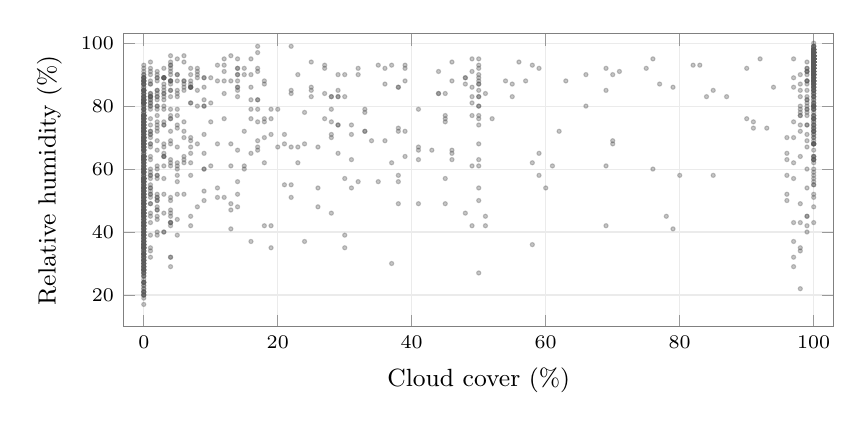
\begin{tikzpicture}
\begin{axis}[width=10.6cm,height=5.3cm,xlabel={Cloud cover (\%)},ylabel={Relative humidity (\%)},xmin=-3,xmax=103,ymin=10,ymax=103]
\addplot[only marks,mark=*,mark size=0.75pt,color=black!65,opacity=0.34] coordinates {
(61.00000,61.00000)
(28.00000,71.00000)
(49.00000,77.00000)
(14.00000,83.00000)
(50.00000,85.00000)
(0.00000,89.00000)
(15.00000,90.00000)
(27.00000,93.00000)
(12.00000,95.00000)
(14.00000,95.00000)
(14.00000,92.00000)
(100.00000,92.00000)
(100.00000,92.00000)
(100.00000,92.00000)
(8.00000,80.00000)
(14.00000,88.00000)
(100.00000,83.00000)
(100.00000,76.00000)
(100.00000,73.00000)
(100.00000,75.00000)
(21.00000,71.00000)
(99.00000,79.00000)
(99.00000,82.00000)
(0.00000,81.00000)
(4.00000,79.00000)
(50.00000,83.00000)
(100.00000,91.00000)
(100.00000,95.00000)
(100.00000,97.00000)
(13.00000,96.00000)
(100.00000,95.00000)
(100.00000,94.00000)
(100.00000,97.00000)
(100.00000,93.00000)
(100.00000,91.00000)
(100.00000,92.00000)
(100.00000,96.00000)
(100.00000,97.00000)
(100.00000,94.00000)
(100.00000,92.00000)
(100.00000,90.00000)
(100.00000,88.00000)
(100.00000,95.00000)
(100.00000,94.00000)
(100.00000,86.00000)
(100.00000,84.00000)
(57.00000,88.00000)
(100.00000,90.00000)
(100.00000,93.00000)
(100.00000,94.00000)
(100.00000,96.00000)
(100.00000,93.00000)
(100.00000,93.00000)
(100.00000,94.00000)
(100.00000,95.00000)
(100.00000,96.00000)
(100.00000,97.00000)
(100.00000,97.00000)
(100.00000,98.00000)
(100.00000,97.00000)
(17.00000,99.00000)
(100.00000,96.00000)
(100.00000,92.00000)
(100.00000,80.00000)
(29.00000,74.00000)
(28.00000,70.00000)
(22.00000,67.00000)
(15.00000,61.00000)
(100.00000,57.00000)
(9.00000,60.00000)
(15.00000,72.00000)
(33.00000,72.00000)
(7.00000,87.00000)
(4.00000,96.00000)
(0.00000,92.00000)
(1.00000,91.00000)
(0.00000,85.00000)
(0.00000,85.00000)
(0.00000,79.00000)
(0.00000,82.00000)
(0.00000,80.00000)
(0.00000,74.00000)
(0.00000,77.00000)
(0.00000,81.00000)
(4.00000,93.00000)
(7.00000,86.00000)
(4.00000,76.00000)
(6.00000,64.00000)
(9.00000,60.00000)
(38.00000,58.00000)
(12.00000,51.00000)
(26.00000,48.00000)
(7.00000,45.00000)
(1.00000,46.00000)
(0.00000,46.00000)
(0.00000,57.00000)
(2.00000,60.00000)
(0.00000,62.00000)
(0.00000,63.00000)
(0.00000,68.00000)
(0.00000,78.00000)
(0.00000,82.00000)
(0.00000,85.00000)
(3.00000,89.00000)
(3.00000,89.00000)
(5.00000,88.00000)
(3.00000,89.00000)
(3.00000,89.00000)
(6.00000,96.00000)
(0.00000,77.00000)
(3.00000,68.00000)
(1.00000,52.00000)
(4.00000,47.00000)
(3.00000,46.00000)
(5.00000,44.00000)
(4.00000,43.00000)
(2.00000,44.00000)
(0.00000,45.00000)
(0.00000,50.00000)
(0.00000,58.00000)
(0.00000,66.00000)
(0.00000,73.00000)
(0.00000,82.00000)
(0.00000,85.00000)
(0.00000,83.00000)
(0.00000,82.00000)
(50.00000,87.00000)
(48.00000,89.00000)
(1.00000,87.00000)
(4.00000,88.00000)
(2.00000,89.00000)
(1.00000,92.00000)
(4.00000,94.00000)
(4.00000,88.00000)
(4.00000,76.00000)
(1.00000,64.00000)
(0.00000,57.00000)
(0.00000,56.00000)
(1.00000,54.00000)
(0.00000,55.00000)
(0.00000,55.00000)
(0.00000,57.00000)
(0.00000,54.00000)
(0.00000,60.00000)
(0.00000,69.00000)
(0.00000,75.00000)
(0.00000,86.00000)
(59.00000,92.00000)
(32.00000,92.00000)
(0.00000,89.00000)
(0.00000,87.00000)
(0.00000,89.00000)
(0.00000,88.00000)
(4.00000,92.00000)
(0.00000,88.00000)
(0.00000,81.00000)
(0.00000,72.00000)
(20.00000,67.00000)
(0.00000,60.00000)
(46.00000,65.00000)
(45.00000,57.00000)
(38.00000,56.00000)
(0.00000,51.00000)
(2.00000,47.00000)
(100.00000,92.00000)
(100.00000,93.00000)
(100.00000,92.00000)
(100.00000,95.00000)
(92.00000,95.00000)
(100.00000,95.00000)
(100.00000,94.00000)
(39.00000,88.00000)
(29.00000,83.00000)
(49.00000,81.00000)
(2.00000,80.00000)
(16.00000,79.00000)
(99.00000,81.00000)
(3.00000,85.00000)
(27.00000,84.00000)
(29.00000,83.00000)
(50.00000,90.00000)
(32.00000,90.00000)
(49.00000,83.00000)
(3.00000,74.00000)
(100.00000,68.00000)
(41.00000,67.00000)
(19.00000,71.00000)
(100.00000,82.00000)
(50.00000,68.00000)
(16.00000,65.00000)
(18.00000,75.00000)
(33.00000,72.00000)
(16.00000,76.00000)
(14.00000,86.00000)
(8.00000,91.00000)
(46.00000,88.00000)
(49.00000,95.00000)
(56.00000,94.00000)
(100.00000,90.00000)
(100.00000,91.00000)
(14.00000,92.00000)
(100.00000,83.00000)
(100.00000,86.00000)
(38.00000,86.00000)
(100.00000,80.00000)
(100.00000,76.00000)
(100.00000,74.00000)
(18.00000,76.00000)
(21.00000,68.00000)
(24.00000,68.00000)
(29.00000,65.00000)
(31.00000,63.00000)
(10.00000,61.00000)
(5.00000,61.00000)
(0.00000,63.00000)
(0.00000,68.00000)
(4.00000,77.00000)
(100.00000,80.00000)
(100.00000,80.00000)
(100.00000,87.00000)
(100.00000,84.00000)
(100.00000,85.00000)
(100.00000,75.00000)
(100.00000,76.00000)
(1.00000,80.00000)
(0.00000,77.00000)
(0.00000,84.00000)
(13.00000,88.00000)
(100.00000,92.00000)
(66.00000,90.00000)
(41.00000,79.00000)
(31.00000,74.00000)
(23.00000,67.00000)
(58.00000,62.00000)
(15.00000,60.00000)
(80.00000,58.00000)
(100.00000,58.00000)
(39.00000,64.00000)
(70.00000,68.00000)
(5.00000,67.00000)
(6.00000,75.00000)
(85.00000,85.00000)
(8.00000,90.00000)
(63.00000,88.00000)
(69.00000,92.00000)
(18.00000,87.00000)
(1.00000,88.00000)
(0.00000,88.00000)
(4.00000,91.00000)
(7.00000,92.00000)
(0.00000,91.00000)
(3.00000,92.00000)
(25.00000,94.00000)
(100.00000,90.00000)
(100.00000,87.00000)
(100.00000,90.00000)
(100.00000,85.00000)
(100.00000,86.00000)
(100.00000,83.00000)
(100.00000,84.00000)
(100.00000,86.00000)
(100.00000,82.00000)
(100.00000,88.00000)
(100.00000,93.00000)
(100.00000,93.00000)
(100.00000,92.00000)
(100.00000,92.00000)
(100.00000,96.00000)
(100.00000,94.00000)
(100.00000,96.00000)
(100.00000,96.00000)
(100.00000,96.00000)
(100.00000,95.00000)
(100.00000,96.00000)
(100.00000,95.00000)
(100.00000,93.00000)
(100.00000,96.00000)
(100.00000,94.00000)
(100.00000,96.00000)
(100.00000,90.00000)
(100.00000,95.00000)
(100.00000,91.00000)
(100.00000,89.00000)
(100.00000,97.00000)
(100.00000,93.00000)
(100.00000,94.00000)
(100.00000,96.00000)
(100.00000,97.00000)
(100.00000,96.00000)
(100.00000,95.00000)
(100.00000,95.00000)
(100.00000,95.00000)
(100.00000,95.00000)
(100.00000,96.00000)
(100.00000,96.00000)
(100.00000,95.00000)
(100.00000,93.00000)
(100.00000,92.00000)
(100.00000,93.00000)
(100.00000,93.00000)
(100.00000,92.00000)
(100.00000,98.00000)
(100.00000,95.00000)
(100.00000,95.00000)
(100.00000,95.00000)
(100.00000,95.00000)
(100.00000,96.00000)
(100.00000,97.00000)
(100.00000,96.00000)
(100.00000,93.00000)
(100.00000,92.00000)
(100.00000,91.00000)
(100.00000,93.00000)
(1.00000,94.00000)
(100.00000,90.00000)
(50.00000,88.00000)
(25.00000,86.00000)
(44.00000,84.00000)
(30.00000,83.00000)
(100.00000,81.00000)
(33.00000,78.00000)
(50.00000,80.00000)
(9.00000,80.00000)
(100.00000,79.00000)
(100.00000,80.00000)
(100.00000,78.00000)
(100.00000,79.00000)
(50.00000,76.00000)
(31.00000,71.00000)
(7.00000,70.00000)
(100.00000,63.00000)
(100.00000,63.00000)
(100.00000,60.00000)
(13.00000,61.00000)
(17.00000,67.00000)
(2.00000,66.00000)
(2.00000,77.00000)
(3.00000,82.00000)
(0.00000,87.00000)
(17.00000,92.00000)
(5.00000,90.00000)
(10.00000,89.00000)
(100.00000,92.00000)
(44.00000,91.00000)
(7.00000,86.00000)
(1.00000,82.00000)
(0.00000,77.00000)
(0.00000,75.00000)
(0.00000,77.00000)
(0.00000,73.00000)
(0.00000,51.00000)
(0.00000,37.00000)
(0.00000,33.00000)
(0.00000,33.00000)
(0.00000,29.00000)
(0.00000,22.00000)
(0.00000,22.00000)
(98.00000,22.00000)
(0.00000,23.00000)
(0.00000,26.00000)
(0.00000,29.00000)
(49.00000,42.00000)
(0.00000,51.00000)
(0.00000,51.00000)
(0.00000,47.00000)
(0.00000,50.00000)
(0.00000,49.00000)
(0.00000,52.00000)
(0.00000,57.00000)
(0.00000,57.00000)
(0.00000,57.00000)
(0.00000,56.00000)
(0.00000,53.00000)
(0.00000,47.00000)
(0.00000,40.00000)
(0.00000,38.00000)
(0.00000,39.00000)
(0.00000,37.00000)
(0.00000,31.00000)
(4.00000,29.00000)
(1.00000,32.00000)
(0.00000,28.00000)
(0.00000,27.00000)
(0.00000,27.00000)
(100.00000,59.00000)
(100.00000,64.00000)
(97.00000,89.00000)
(100.00000,89.00000)
(77.00000,87.00000)
(84.00000,83.00000)
(5.00000,73.00000)
(4.00000,68.00000)
(14.00000,66.00000)
(39.00000,72.00000)
(38.00000,73.00000)
(3.00000,75.00000)
(7.00000,69.00000)
(26.00000,67.00000)
(50.00000,61.00000)
(21.00000,55.00000)
(1.00000,54.00000)
(45.00000,49.00000)
(100.00000,48.00000)
(69.00000,42.00000)
(58.00000,36.00000)
(97.00000,43.00000)
(100.00000,52.00000)
(99.00000,54.00000)
(49.00000,61.00000)
(50.00000,54.00000)
(7.00000,58.00000)
(46.00000,63.00000)
(23.00000,62.00000)
(3.00000,67.00000)
(2.00000,72.00000)
(0.00000,79.00000)
(28.00000,75.00000)
(18.00000,70.00000)
(0.00000,77.00000)
(50.00000,77.00000)
(50.00000,80.00000)
(28.00000,83.00000)
(38.00000,72.00000)
(50.00000,63.00000)
(30.00000,57.00000)
(100.00000,55.00000)
(32.00000,56.00000)
(50.00000,50.00000)
(22.00000,51.00000)
(9.00000,50.00000)
(59.00000,58.00000)
(18.00000,62.00000)
(100.00000,68.00000)
(100.00000,77.00000)
(100.00000,80.00000)
(100.00000,72.00000)
(100.00000,71.00000)
(100.00000,74.00000)
(100.00000,90.00000)
(45.00000,84.00000)
(22.00000,85.00000)
(4.00000,88.00000)
(7.00000,86.00000)
(79.00000,86.00000)
(50.00000,92.00000)
(14.00000,85.00000)
(12.00000,76.00000)
(36.00000,69.00000)
(41.00000,66.00000)
(100.00000,68.00000)
(100.00000,68.00000)
(96.00000,70.00000)
(17.00000,66.00000)
(6.00000,62.00000)
(4.00000,63.00000)
(0.00000,70.00000)
(0.00000,74.00000)
(0.00000,81.00000)
(0.00000,84.00000)
(4.00000,90.00000)
(9.00000,89.00000)
(37.00000,93.00000)
(48.00000,89.00000)
(30.00000,90.00000)
(7.00000,86.00000)
(4.00000,85.00000)
(4.00000,88.00000)
(2.00000,89.00000)
(0.00000,93.00000)
(50.00000,95.00000)
(2.00000,85.00000)
(2.00000,73.00000)
(3.00000,64.00000)
(26.00000,54.00000)
(4.00000,46.00000)
(51.00000,45.00000)
(4.00000,43.00000)
(18.00000,42.00000)
(38.00000,49.00000)
(8.00000,68.00000)
(66.00000,80.00000)
(14.00000,86.00000)
(51.00000,84.00000)
(0.00000,83.00000)
(1.00000,83.00000)
(2.00000,88.00000)
(0.00000,81.00000)
(20.00000,79.00000)
(29.00000,90.00000)
(0.00000,88.00000)
(0.00000,85.00000)
(0.00000,89.00000)
(14.00000,90.00000)
(16.00000,82.00000)
(3.00000,64.00000)
(0.00000,54.00000)
(0.00000,46.00000)
(0.00000,39.00000)
(0.00000,36.00000)
(0.00000,33.00000)
(0.00000,28.00000)
(0.00000,30.00000)
(4.00000,32.00000)
(0.00000,47.00000)
(0.00000,57.00000)
(0.00000,63.00000)
(0.00000,61.00000)
(0.00000,68.00000)
(0.00000,70.00000)
(0.00000,73.00000)
(0.00000,72.00000)
(0.00000,70.00000)
(1.00000,67.00000)
(1.00000,76.00000)
(0.00000,77.00000)
(0.00000,83.00000)
(0.00000,81.00000)
(0.00000,71.00000)
(11.00000,51.00000)
(0.00000,47.00000)
(0.00000,45.00000)
(0.00000,45.00000)
(1.00000,39.00000)
(13.00000,41.00000)
(30.00000,39.00000)
(51.00000,42.00000)
(28.00000,46.00000)
(8.00000,48.00000)
(100.00000,70.00000)
(100.00000,69.00000)
(25.00000,85.00000)
(71.00000,91.00000)
(27.00000,92.00000)
(100.00000,90.00000)
(100.00000,85.00000)
(100.00000,74.00000)
(100.00000,80.00000)
(100.00000,88.00000)
(100.00000,95.00000)
(100.00000,94.00000)
(100.00000,95.00000)
(100.00000,96.00000)
(100.00000,96.00000)
(100.00000,98.00000)
(100.00000,95.00000)
(99.00000,94.00000)
(99.00000,92.00000)
(100.00000,92.00000)
(100.00000,95.00000)
(100.00000,94.00000)
(100.00000,94.00000)
(100.00000,97.00000)
(100.00000,97.00000)
(100.00000,97.00000)
(100.00000,97.00000)
(100.00000,96.00000)
(100.00000,98.00000)
(100.00000,96.00000)
(100.00000,98.00000)
(100.00000,99.00000)
(100.00000,97.00000)
(100.00000,98.00000)
(100.00000,98.00000)
(100.00000,98.00000)
(100.00000,97.00000)
(100.00000,95.00000)
(100.00000,99.00000)
(100.00000,98.00000)
(100.00000,98.00000)
(100.00000,94.00000)
(100.00000,92.00000)
(100.00000,88.00000)
(100.00000,89.00000)
(100.00000,88.00000)
(100.00000,88.00000)
(100.00000,87.00000)
(100.00000,91.00000)
(100.00000,93.00000)
(100.00000,94.00000)
(100.00000,94.00000)
(97.00000,95.00000)
(100.00000,94.00000)
(100.00000,97.00000)
(100.00000,97.00000)
(100.00000,95.00000)
(100.00000,98.00000)
(100.00000,97.00000)
(100.00000,95.00000)
(100.00000,99.00000)
(100.00000,94.00000)
(50.00000,87.00000)
(29.00000,74.00000)
(0.00000,54.00000)
(1.00000,49.00000)
(2.00000,40.00000)
(3.00000,40.00000)
(1.00000,35.00000)
(0.00000,34.00000)
(0.00000,34.00000)
(0.00000,51.00000)
(0.00000,52.00000)
(0.00000,60.00000)
(0.00000,66.00000)
(0.00000,64.00000)
(0.00000,57.00000)
(0.00000,70.00000)
(0.00000,81.00000)
(0.00000,75.00000)
(0.00000,72.00000)
(0.00000,76.00000)
(0.00000,84.00000)
(1.00000,87.00000)
(5.00000,95.00000)
(0.00000,79.00000)
(0.00000,53.00000)
(0.00000,45.00000)
(0.00000,41.00000)
(0.00000,38.00000)
(0.00000,35.00000)
(0.00000,36.00000)
(0.00000,35.00000)
(0.00000,35.00000)
(0.00000,39.00000)
(0.00000,54.00000)
(0.00000,64.00000)
(1.00000,79.00000)
(12.00000,88.00000)
(9.00000,89.00000)
(99.00000,92.00000)
(75.00000,92.00000)
(58.00000,93.00000)
(82.00000,93.00000)
(49.00000,91.00000)
(100.00000,93.00000)
(100.00000,94.00000)
(2.00000,90.00000)
(0.00000,90.00000)
(0.00000,87.00000)
(1.00000,84.00000)
(2.00000,69.00000)
(1.00000,59.00000)
(2.00000,51.00000)
(2.00000,51.00000)
(2.00000,50.00000)
(0.00000,44.00000)
(0.00000,41.00000)
(0.00000,45.00000)
(0.00000,59.00000)
(0.00000,69.00000)
(0.00000,76.00000)
(0.00000,76.00000)
(0.00000,74.00000)
(0.00000,75.00000)
(0.00000,65.00000)
(0.00000,66.00000)
(0.00000,67.00000)
(0.00000,64.00000)
(0.00000,56.00000)
(0.00000,63.00000)
(4.00000,62.00000)
(0.00000,64.00000)
(0.00000,67.00000)
(0.00000,51.00000)
(0.00000,46.00000)
(0.00000,43.00000)
(0.00000,39.00000)
(1.00000,34.00000)
(0.00000,35.00000)
(0.00000,32.00000)
(4.00000,32.00000)
(0.00000,30.00000)
(0.00000,40.00000)
(0.00000,47.00000)
(0.00000,57.00000)
(0.00000,52.00000)
(96.00000,58.00000)
(96.00000,52.00000)
(96.00000,50.00000)
(96.00000,63.00000)
(96.00000,65.00000)
(97.00000,62.00000)
(97.00000,70.00000)
(91.00000,75.00000)
(100.00000,79.00000)
(98.00000,78.00000)
(97.00000,86.00000)
(97.00000,57.00000)
(78.00000,45.00000)
(97.00000,37.00000)
(97.00000,32.00000)
(97.00000,29.00000)
(98.00000,34.00000)
(98.00000,35.00000)
(98.00000,43.00000)
(98.00000,49.00000)
(98.00000,64.00000)
(98.00000,74.00000)
(98.00000,72.00000)
(98.00000,83.00000)
(98.00000,79.00000)
(99.00000,88.00000)
(98.00000,90.00000)
(55.00000,87.00000)
(98.00000,85.00000)
(98.00000,87.00000)
(100.00000,92.00000)
(100.00000,95.00000)
(99.00000,91.00000)
(99.00000,91.00000)
(99.00000,88.00000)
(99.00000,85.00000)
(99.00000,78.00000)
(99.00000,77.00000)
(99.00000,67.00000)
(41.00000,63.00000)
(85.00000,58.00000)
(100.00000,64.00000)
(100.00000,51.00000)
(100.00000,68.00000)
(100.00000,73.00000)
(100.00000,77.00000)
(100.00000,72.00000)
(100.00000,73.00000)
(100.00000,72.00000)
(100.00000,85.00000)
(100.00000,92.00000)
(100.00000,91.00000)
(100.00000,92.00000)
(100.00000,95.00000)
(100.00000,95.00000)
(100.00000,96.00000)
(100.00000,94.00000)
(100.00000,94.00000)
(100.00000,96.00000)
(100.00000,94.00000)
(100.00000,97.00000)
(100.00000,96.00000)
(100.00000,97.00000)
(100.00000,96.00000)
(100.00000,97.00000)
(100.00000,94.00000)
(100.00000,93.00000)
(100.00000,95.00000)
(100.00000,95.00000)
(100.00000,94.00000)
(100.00000,95.00000)
(100.00000,97.00000)
(100.00000,98.00000)
(100.00000,98.00000)
(100.00000,97.00000)
(100.00000,95.00000)
(46.00000,94.00000)
(0.00000,89.00000)
(100.00000,87.00000)
(0.00000,88.00000)
(1.00000,82.00000)
(0.00000,81.00000)
(0.00000,87.00000)
(0.00000,76.00000)
(0.00000,64.00000)
(0.00000,60.00000)
(0.00000,57.00000)
(0.00000,55.00000)
(1.00000,55.00000)
(5.00000,52.00000)
(0.00000,54.00000)
(1.00000,60.00000)
(6.00000,70.00000)
(0.00000,67.00000)
(0.00000,77.00000)
(0.00000,74.00000)
(2.00000,75.00000)
(6.00000,85.00000)
(7.00000,90.00000)
(100.00000,93.00000)
(100.00000,94.00000)
(3.00000,87.00000)
(0.00000,77.00000)
(0.00000,70.00000)
(0.00000,62.00000)
(0.00000,74.00000)
(0.00000,82.00000)
(0.00000,74.00000)
(0.00000,60.00000)
(0.00000,50.00000)
(0.00000,47.00000)
(0.00000,45.00000)
(0.00000,40.00000)
(0.00000,44.00000)
(0.00000,43.00000)
(0.00000,48.00000)
(0.00000,65.00000)
(0.00000,70.00000)
(0.00000,77.00000)
(0.00000,73.00000)
(0.00000,71.00000)
(0.00000,69.00000)
(0.00000,69.00000)
(0.00000,64.00000)
(0.00000,62.00000)
(0.00000,62.00000)
(0.00000,64.00000)
(0.00000,67.00000)
(0.00000,63.00000)
(2.00000,61.00000)
(0.00000,64.00000)
(0.00000,63.00000)
(0.00000,52.00000)
(0.00000,48.00000)
(0.00000,48.00000)
(0.00000,46.00000)
(0.00000,47.00000)
(0.00000,46.00000)
(0.00000,44.00000)
(13.00000,47.00000)
(2.00000,58.00000)
(0.00000,60.00000)
(3.00000,64.00000)
(59.00000,65.00000)
(99.00000,74.00000)
(100.00000,88.00000)
(100.00000,88.00000)
(12.00000,91.00000)
(0.00000,90.00000)
(100.00000,88.00000)
(49.00000,86.00000)
(18.00000,88.00000)
(83.00000,93.00000)
(100.00000,89.00000)
(100.00000,91.00000)
(100.00000,88.00000)
(100.00000,93.00000)
(100.00000,96.00000)
(100.00000,92.00000)
(100.00000,90.00000)
(100.00000,93.00000)
(100.00000,87.00000)
(100.00000,88.00000)
(100.00000,90.00000)
(100.00000,92.00000)
(100.00000,93.00000)
(100.00000,93.00000)
(100.00000,95.00000)
(100.00000,95.00000)
(100.00000,95.00000)
(100.00000,96.00000)
(100.00000,95.00000)
(100.00000,95.00000)
(100.00000,96.00000)
(100.00000,98.00000)
(100.00000,94.00000)
(100.00000,96.00000)
(100.00000,97.00000)
(100.00000,95.00000)
(100.00000,92.00000)
(8.00000,89.00000)
(5.00000,84.00000)
(5.00000,79.00000)
(0.00000,72.00000)
(0.00000,67.00000)
(1.00000,58.00000)
(1.00000,57.00000)
(1.00000,63.00000)
(9.00000,65.00000)
(99.00000,60.00000)
(34.00000,69.00000)
(99.00000,69.00000)
(100.00000,66.00000)
(100.00000,63.00000)
(100.00000,63.00000)
(100.00000,64.00000)
(100.00000,71.00000)
(100.00000,76.00000)
(100.00000,90.00000)
(100.00000,86.00000)
(100.00000,87.00000)
(98.00000,77.00000)
(94.00000,86.00000)
(99.00000,79.00000)
(98.00000,80.00000)
(43.00000,66.00000)
(100.00000,56.00000)
(13.00000,49.00000)
(19.00000,42.00000)
(0.00000,39.00000)
(0.00000,36.00000)
(0.00000,35.00000)
(0.00000,45.00000)
(0.00000,55.00000)
(0.00000,61.00000)
(0.00000,66.00000)
(0.00000,68.00000)
(0.00000,63.00000)
(0.00000,64.00000)
(0.00000,70.00000)
(0.00000,75.00000)
(0.00000,62.00000)
(0.00000,66.00000)
(0.00000,76.00000)
(0.00000,76.00000)
(0.00000,75.00000)
(0.00000,68.00000)
(0.00000,57.00000)
(0.00000,43.00000)
(0.00000,35.00000)
(0.00000,28.00000)
(0.00000,21.00000)
(0.00000,21.00000)
(0.00000,17.00000)
(0.00000,19.00000)
(0.00000,30.00000)
(0.00000,35.00000)
(0.00000,50.00000)
(0.00000,62.00000)
(0.00000,73.00000)
(0.00000,81.00000)
(3.00000,89.00000)
(17.00000,91.00000)
(69.00000,85.00000)
(24.00000,78.00000)
(1.00000,81.00000)
(2.00000,85.00000)
(9.00000,82.00000)
(3.00000,83.00000)
(2.00000,83.00000)
(0.00000,83.00000)
(0.00000,63.00000)
(0.00000,46.00000)
(0.00000,32.00000)
(0.00000,31.00000)
(0.00000,29.00000)
(0.00000,25.00000)
(0.00000,24.00000)
(0.00000,24.00000)
(0.00000,27.00000)
(0.00000,34.00000)
(0.00000,44.00000)
(0.00000,53.00000)
(0.00000,56.00000)
(0.00000,54.00000)
(0.00000,58.00000)
(0.00000,55.00000)
(0.00000,59.00000)
(0.00000,71.00000)
(0.00000,71.00000)
(0.00000,64.00000)
(0.00000,59.00000)
(0.00000,56.00000)
(0.00000,53.00000)
(0.00000,55.00000)
(0.00000,50.00000)
(0.00000,42.00000)
(0.00000,30.00000)
(0.00000,30.00000)
(0.00000,31.00000)
(0.00000,29.00000)
(0.00000,28.00000)
(0.00000,27.00000)
(0.00000,30.00000)
(0.00000,41.00000)
(0.00000,52.00000)
(0.00000,64.00000)
(0.00000,64.00000)
(0.00000,68.00000)
(0.00000,68.00000)
(0.00000,73.00000)
(0.00000,69.00000)
(0.00000,66.00000)
(0.00000,69.00000)
(0.00000,69.00000)
(0.00000,68.00000)
(1.00000,72.00000)
(0.00000,70.00000)
(0.00000,72.00000)
(0.00000,52.00000)
(0.00000,41.00000)
(0.00000,40.00000)
(0.00000,36.00000)
(0.00000,34.00000)
(0.00000,32.00000)
(0.00000,33.00000)
(0.00000,33.00000)
(0.00000,36.00000)
(0.00000,46.00000)
(0.00000,51.00000)
(0.00000,57.00000)
(0.00000,71.00000)
(0.00000,72.00000)
(0.00000,69.00000)
(1.00000,81.00000)
(0.00000,70.00000)
(0.00000,67.00000)
(0.00000,69.00000)
(0.00000,68.00000)
(1.00000,71.00000)
(1.00000,72.00000)
(1.00000,70.00000)
(0.00000,68.00000)
(0.00000,60.00000)
(0.00000,46.00000)
(0.00000,36.00000)
(0.00000,31.00000)
(0.00000,28.00000)
(0.00000,24.00000)
(0.00000,21.00000)
(0.00000,21.00000)
(0.00000,24.00000)
(0.00000,36.00000)
(0.00000,40.00000)
(0.00000,44.00000)
(0.00000,52.00000)
(0.00000,52.00000)
(0.00000,56.00000)
(0.00000,59.00000)
(0.00000,53.00000)
(0.00000,53.00000)
(0.00000,53.00000)
(0.00000,57.00000)
(1.00000,68.00000)
(0.00000,67.00000)
(0.00000,72.00000)
(0.00000,72.00000)
(3.00000,61.00000)
(3.00000,57.00000)
(1.00000,53.00000)
(100.00000,55.00000)
(0.00000,47.00000)
(100.00000,43.00000)
(2.00000,45.00000)
(0.00000,43.00000)
(0.00000,45.00000)
(0.00000,56.00000)
(0.00000,63.00000)
(0.00000,74.00000)
(1.00000,83.00000)
(0.00000,83.00000)
(0.00000,87.00000)
(4.00000,93.00000)
(0.00000,85.00000)
(4.00000,87.00000)
(1.00000,84.00000)
(4.00000,85.00000)
(5.00000,85.00000)
(9.00000,86.00000)
(6.00000,87.00000)
(17.00000,97.00000)
(29.00000,85.00000)
(4.00000,69.00000)
(2.00000,52.00000)
(0.00000,48.00000)
(4.00000,43.00000)
(2.00000,39.00000)
(7.00000,42.00000)
(4.00000,45.00000)
(0.00000,46.00000)
(0.00000,51.00000)
(7.00000,67.00000)
(4.00000,72.00000)
(1.00000,83.00000)
(1.00000,83.00000)
(3.00000,84.00000)
(100.00000,91.00000)
(100.00000,97.00000)
(100.00000,95.00000)
(100.00000,99.00000)
(100.00000,97.00000)
(100.00000,95.00000)
(6.00000,88.00000)
(7.00000,88.00000)
(3.00000,89.00000)
(45.00000,75.00000)
(5.00000,62.00000)
(2.00000,58.00000)
(1.00000,52.00000)
(4.00000,51.00000)
(1.00000,49.00000)
(2.00000,47.00000)
(0.00000,46.00000)
(0.00000,52.00000)
(0.00000,65.00000)
(0.00000,76.00000)
(3.00000,74.00000)
(45.00000,76.00000)
(9.00000,80.00000)
(0.00000,75.00000)
(0.00000,77.00000)
(0.00000,76.00000)
(0.00000,74.00000)
(0.00000,77.00000)
(0.00000,73.00000)
(0.00000,73.00000)
(5.00000,74.00000)
(0.00000,84.00000)
(0.00000,88.00000)
(0.00000,85.00000)
(0.00000,76.00000)
(0.00000,61.00000)
(0.00000,49.00000)
(0.00000,39.00000)
(0.00000,37.00000)
(0.00000,37.00000)
(0.00000,39.00000)
(0.00000,43.00000)
(0.00000,54.00000)
(0.00000,67.00000)
(0.00000,70.00000)
(0.00000,79.00000)
(1.00000,80.00000)
(0.00000,64.00000)
(0.00000,47.00000)
(0.00000,57.00000)
(4.00000,61.00000)
(0.00000,63.00000)
(0.00000,68.00000)
(0.00000,71.00000)
(2.00000,74.00000)
(0.00000,73.00000)
(0.00000,72.00000)
(0.00000,63.00000)
(0.00000,54.00000)
(0.00000,49.00000)
(0.00000,46.00000)
(0.00000,46.00000)
(1.00000,45.00000)
(0.00000,43.00000)
(0.00000,42.00000)
(0.00000,43.00000)
(0.00000,49.00000)
(0.00000,60.00000)
(6.00000,86.00000)
(48.00000,87.00000)
(38.00000,86.00000)
(36.00000,87.00000)
(7.00000,86.00000)
(0.00000,80.00000)
(5.00000,83.00000)
(25.00000,83.00000)
(100.00000,89.00000)
(100.00000,96.00000)
(50.00000,93.00000)
(100.00000,95.00000)
(100.00000,100.00000)
(100.00000,95.00000)
(54.00000,88.00000)
(33.00000,79.00000)
(99.00000,71.00000)
(99.00000,74.00000)
(93.00000,73.00000)
(100.00000,72.00000)
(90.00000,76.00000)
(50.00000,74.00000)
(45.00000,77.00000)
(2.00000,84.00000)
(44.00000,84.00000)
(50.00000,89.00000)
(35.00000,93.00000)
(100.00000,96.00000)
(100.00000,91.00000)
(100.00000,90.00000)
(8.00000,92.00000)
(100.00000,94.00000)
(100.00000,97.00000)
(100.00000,97.00000)
(39.00000,93.00000)
(36.00000,92.00000)
(22.00000,99.00000)
(6.00000,88.00000)
(1.00000,74.00000)
(6.00000,63.00000)
(5.00000,58.00000)
(2.00000,50.00000)
(0.00000,45.00000)
(0.00000,42.00000)
(0.00000,47.00000)
(0.00000,49.00000)
(0.00000,63.00000)
(0.00000,74.00000)
(0.00000,78.00000)
(0.00000,77.00000)
(0.00000,75.00000)
(0.00000,77.00000)
(0.00000,72.00000)
(0.00000,59.00000)
(0.00000,50.00000)
(0.00000,54.00000)
(0.00000,56.00000)
(0.00000,64.00000)
(0.00000,61.00000)
(4.00000,50.00000)
(0.00000,56.00000)
(0.00000,48.00000)
(0.00000,42.00000)
(0.00000,38.00000)
(0.00000,33.00000)
(0.00000,28.00000)
(0.00000,23.00000)
(0.00000,20.00000)
(0.00000,20.00000)
(0.00000,20.00000)
(0.00000,29.00000)
(0.00000,31.00000)
(0.00000,35.00000)
(0.00000,42.00000)
(2.00000,48.00000)
(0.00000,49.00000)
(0.00000,54.00000)
(0.00000,60.00000)
(0.00000,57.00000)
(0.00000,70.00000)
(0.00000,69.00000)
(17.00000,69.00000)
(0.00000,66.00000)
(9.00000,71.00000)
(0.00000,80.00000)
(1.00000,68.00000)
(2.00000,57.00000)
(11.00000,54.00000)
(41.00000,49.00000)
(99.00000,45.00000)
(99.00000,42.00000)
(79.00000,41.00000)
(99.00000,40.00000)
(99.00000,45.00000)
(22.00000,55.00000)
(69.00000,61.00000)
(46.00000,66.00000)
(91.00000,73.00000)
(98.00000,77.00000)
(99.00000,80.00000)
(17.00000,79.00000)
(3.00000,80.00000)
(2.00000,79.00000)
(5.00000,77.00000)
(28.00000,79.00000)
(28.00000,83.00000)
(10.00000,75.00000)
(2.00000,80.00000)
(0.00000,82.00000)
(0.00000,71.00000)
(1.00000,58.00000)
(0.00000,40.00000)
(0.00000,37.00000)
(0.00000,31.00000)
(0.00000,29.00000)
(50.00000,27.00000)
(37.00000,30.00000)
(19.00000,35.00000)
(14.00000,48.00000)
(0.00000,51.00000)
(76.00000,60.00000)
(3.00000,65.00000)
(13.00000,68.00000)
(17.00000,75.00000)
(17.00000,82.00000)
(8.00000,85.00000)
(99.00000,91.00000)
(99.00000,87.00000)
(99.00000,90.00000)
(99.00000,82.00000)
(99.00000,88.00000)
(87.00000,83.00000)
(99.00000,83.00000)
(70.00000,69.00000)
(37.00000,62.00000)
(48.00000,46.00000)
(0.00000,42.00000)
(5.00000,39.00000)
(4.00000,42.00000)
(3.00000,40.00000)
(24.00000,37.00000)
(0.00000,42.00000)
(1.00000,51.00000)
(5.00000,56.00000)
(0.00000,70.00000)
(0.00000,72.00000)
(0.00000,79.00000)
(2.00000,83.00000)
(19.00000,76.00000)
(0.00000,85.00000)
(0.00000,77.00000)
(0.00000,75.00000)
(0.00000,70.00000)
(0.00000,81.00000)
(50.00000,83.00000)
(0.00000,86.00000)
(7.00000,81.00000)
(1.00000,71.00000)
(7.00000,62.00000)
(31.00000,54.00000)
(0.00000,56.00000)
(0.00000,49.00000)
(0.00000,42.00000)
(0.00000,44.00000)
(0.00000,50.00000)
(0.00000,49.00000)
(0.00000,59.00000)
(0.00000,69.00000)
(0.00000,74.00000)
(0.00000,78.00000)
(0.00000,82.00000)
(0.00000,83.00000)
(0.00000,82.00000)
(0.00000,81.00000)
(2.00000,82.00000)
(1.00000,90.00000)
(12.00000,93.00000)
(11.00000,93.00000)
(2.00000,91.00000)
(5.00000,90.00000)
(6.00000,94.00000)
(10.00000,81.00000)
(11.00000,68.00000)
(5.00000,60.00000)
(0.00000,54.00000)
(6.00000,52.00000)
(14.00000,52.00000)
(14.00000,56.00000)
(3.00000,52.00000)
(60.00000,54.00000)
(62.00000,72.00000)
(3.00000,79.00000)
(19.00000,79.00000)
(55.00000,83.00000)
(70.00000,90.00000)
(100.00000,88.00000)
(100.00000,90.00000)
(100.00000,93.00000)
(100.00000,90.00000)
(100.00000,93.00000)
(100.00000,92.00000)
(100.00000,87.00000)
(100.00000,90.00000)
(39.00000,92.00000)
(14.00000,90.00000)
(100.00000,89.00000)
(100.00000,86.00000)
(100.00000,79.00000)
(100.00000,76.00000)
(100.00000,77.00000)
(100.00000,81.00000)
(100.00000,81.00000)
(100.00000,83.00000)
(100.00000,85.00000)
(100.00000,89.00000)
(100.00000,89.00000)
(16.00000,86.00000)
(3.00000,86.00000)
(3.00000,84.00000)
(1.00000,83.00000)
(100.00000,91.00000)
(100.00000,97.00000)
(76.00000,95.00000)
(100.00000,95.00000)
(100.00000,95.00000)
(100.00000,96.00000)
(16.00000,95.00000)
(23.00000,90.00000)
(90.00000,92.00000)
(17.00000,82.00000)
(6.00000,72.00000)
(100.00000,62.00000)
(100.00000,70.00000)
(100.00000,68.00000)
(97.00000,75.00000)
(0.00000,73.00000)
(0.00000,60.00000)
(0.00000,56.00000)
(0.00000,70.00000)
(7.00000,81.00000)
(16.00000,90.00000)
(15.00000,92.00000)
(22.00000,84.00000)
(4.00000,83.00000)
(12.00000,84.00000)
(11.00000,88.00000)
(52.00000,76.00000)
(27.00000,76.00000)
(7.00000,65.00000)
(0.00000,64.00000)
(0.00000,61.00000)
(0.00000,62.00000)
(0.00000,69.00000)
(0.00000,51.00000)
(0.00000,46.00000)
(0.00000,43.00000)
(0.00000,41.00000)
(0.00000,36.00000)
(0.00000,35.00000)
(0.00000,33.00000)
(0.00000,33.00000)
(0.00000,42.00000)
(0.00000,49.00000)
(0.00000,52.00000)
(0.00000,57.00000)
(0.00000,58.00000)
(0.00000,59.00000)
(0.00000,63.00000)
(0.00000,58.00000)
(0.00000,61.00000)
(0.00000,66.00000)
(0.00000,64.00000)
(0.00000,59.00000)
(0.00000,59.00000)
(0.00000,53.00000)
(0.00000,49.00000)
(0.00000,57.00000)
(0.00000,52.00000)
(0.00000,51.00000)
(0.00000,47.00000)
(0.00000,35.00000)
(0.00000,40.00000)
(0.00000,37.00000)
(0.00000,32.00000)
(0.00000,32.00000)
(0.00000,36.00000)
(0.00000,41.00000)
(0.00000,38.00000)
(0.00000,38.00000)
(0.00000,38.00000)
(16.00000,37.00000)
(0.00000,35.00000)
(30.00000,35.00000)
(0.00000,37.00000)
(0.00000,39.00000)
(0.00000,43.00000)
(0.00000,48.00000)
(0.00000,57.00000)
(35.00000,56.00000)
(9.00000,53.00000)
(0.00000,54.00000)
(0.00000,50.00000)
(1.00000,43.00000)
(0.00000,36.00000)
(0.00000,31.00000)
(0.00000,28.00000)
(0.00000,26.00000)
(0.00000,24.00000)
(0.00000,20.00000)
(0.00000,26.00000)
(0.00000,35.00000)
};
\end{axis}
\end{tikzpicture}
\vspace{-0.3em}
\begin{center}\small Each point is one weather hour. Where would you place the groups?\end{center}
\src{\SnapshotDetails. \DatasetCredit}
\note{Let students describe what they see before introducing the algorithm. Ask how they would distinguish clear, cloudy, and wet conditions from these two measurements. The vertical concentrations at 0 and 100 percent are real features of this model dataset; do not present it as Gaussian blobs.}
\end{frame}

\begin{frame}{What is being clustered?}
\begin{itemize}
\item \textbf{One row:} one hour at a Charlottesville-area grid point.
\item \textbf{Source:} recent hourly weather-model estimates from Open-Meteo.
\item \textbf{Snapshot:} 60 completed UTC days, 1,440 rows, no missing values in the selected features.
\end{itemize}
\vspace{0.4em}
\centering
\small
\begin{tabular}{lrrr}\toprule
UTC hour & Cloud (\%) & Humidity (\%) & Precip. (mm)\\\midrule
2026-09-11 00:00 & 61 & 61 & 0.0\\
2026-09-11 01:00 & 28 & 71 & 0.0\\
2026-09-11 02:00 & 49 & 77 & 0.0\\
2026-09-11 03:00 & 14 & 83 & 0.0\\\bottomrule
\end{tabular}
\vspace{0.4em}
\begin{block}{What these data represent}
Hourly model estimates, not direct station measurements. Precipitation is the preceding hour's total, including rain, showers, and snow water equivalent.
\end{block}
\src{\href{https://open-meteo.com/en/docs}{Open-Meteo API documentation}; retrieved November 10, 2026. Stored times are UTC; the dashboard displays local time.}
\note{Point out the unit of observation. We are clustering hours, not people, days, or locations. Recent values accessed through the forecast API remain model products. The frozen snapshot makes the lecture reproducible; refreshing the dashboard may change the results.}
\end{frame}

\begin{frame}{From predicting labels to discovering patterns}
\begin{columns}[T]
\column{0.48\textwidth}
\begin{block}{Supervised learning}
Observe features $X$ and an outcome $Y$.\\[0.4em]
Learn a rule for predicting $Y$ from $X$.
\end{block}
\column{0.48\textwidth}
\begin{block}{Unsupervised learning}
Observe features $X$.\\[0.4em]
Look for useful structure without supplying an outcome.
\end{block}
\end{columns}
\vspace{0.7em}
\small
\begin{tabular}{L{2.3cm}L{3.7cm}L{3.7cm}}\toprule
& KNN & KMeans\\\midrule
What does $K$ count? & Nearby observations & Cluster centers\\
What is learned? & Predictions from neighbors & Groups and their representatives\\
What do both need? & \multicolumn{2}{l}{Meaningful features, distances, and scaling}\\\bottomrule
\end{tabular}
\note{Use this as the explicit bridge from KNN. K in the two algorithms means different things. KMeans yields numerical cluster identifiers, but those identifiers were not training labels.}
\end{frame}

\begin{frame}{Features define the question}
\begin{block}{Start in two dimensions}
$\xx_i=(\text{cloud cover},\ \text{relative humidity})$.\\
Which hours have similar cloud and moisture conditions?
\end{block}
\begin{block}{Then add a third dimension}
$\xx_i=(\text{cloud cover},\ \text{relative humidity},\ \text{precipitation})$.\\
Does including wetness change the grouping?
\end{block}
\begin{itemize}
\item Weather codes are \textbf{not} used as training labels or features.
\item Time and temperature remain available for later interpretation.
\item $K=3$ is an exploratory choice, not evidence of three true weather types.
\end{itemize}
\note{Ask whether adding temperature would answer the same question. It would make temperature differences part of similarity, possibly changing the grouping. Feature selection is substantive judgment, not just a coding step.}
\end{frame}

\begin{frame}{Scaling changes what ``close'' means}
In raw units, squared distance in three dimensions is
\[
d^2=(\Delta\text{cloud})^2+(\Delta\text{humidity})^2+(\Delta\text{precipitation})^2.
\]
\begin{itemize}
\item A 10-point cloud difference contributes $100$.
\item A 1-mm precipitation difference contributes $1$.
\end{itemize}
\begin{block}{A starting choice: standardize each feature}
\[
z_{ij}=\frac{x_{ij}-\bar x_j}{s_j},\qquad
s_j=\sqrt{\frac1n\sum_{i=1}^n(x_{ij}-\bar x_j)^2}.
\]
One unit is one feature standard deviation. This is the convention used by \texttt{StandardScaler}.
\end{block}
\small Scaling is a modeling choice. Rare large rainfall values can still matter greatly after standardization.
\note{Connect to KNN scaling. Standardization does not make every variable equally informative; it rescales variation. The population-style divisor matches scikit-learn exactly. Comparing raw and scaled SSE numerically is meaningless because the objective's units changed.}
\end{frame}

\begin{frame}{Represent each group by a center}
For cluster $C_k$, the centroid is the coordinatewise mean:
\[
\mm_k=\frac{1}{|C_k|}\sum_{i\in C_k}\xx_i.
\]
\begin{center}
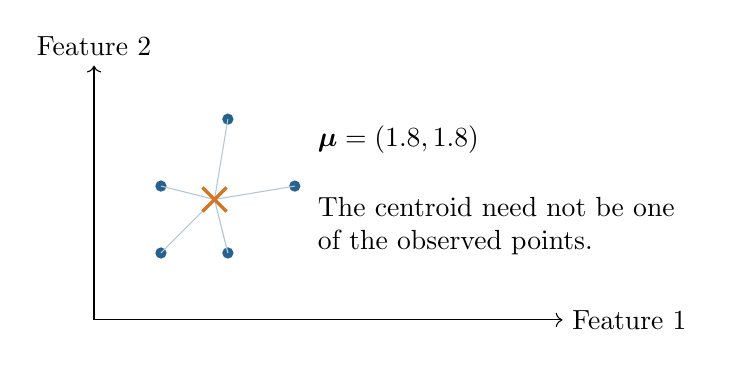
\begin{tikzpicture}[scale=0.85]
\draw[->] (0,0)--(7,0) node[right]{Feature 1};
\draw[->] (0,0)--(0,3.8) node[above]{Feature 2};
\foreach \x/\y in {1/1,1/2,2/1,2/3,3/2} {
\fill[cA] (\x,\y) circle (2.4pt);
\draw[cA!35] (\x,\y)--(1.8,1.8);
}
\draw[very thick,cB] (1.62,1.62)--(1.98,1.98);
\draw[very thick,cB] (1.62,1.98)--(1.98,1.62);
\node[anchor=west] at (3.2,2.7) {$\mm=(1.8,1.8)$};
\node[anchor=west,text width=4.8cm] at (3.2,1.4) {The centroid need not be one of the observed points.};
\end{tikzpicture}
\end{center}
\note{The figure is illustrative, not the weather sample. Interpret the centroid as a representative numerical profile. A real weather hour need not have exactly those values.}
\end{frame}

\begin{frame}{Lloyd's algorithm: assign, average, repeat}
\begin{enumerate}
\item \textbf{Initialize:} choose $K$ starting centers.
\item \textbf{Assign:} put each point in the nearest-center group.
\item \textbf{Update:} replace each center with its group's mean.
\item Repeat assignment and update until the grouping stabilizes.
\end{enumerate}
\vspace{0.6em}
\begin{center}
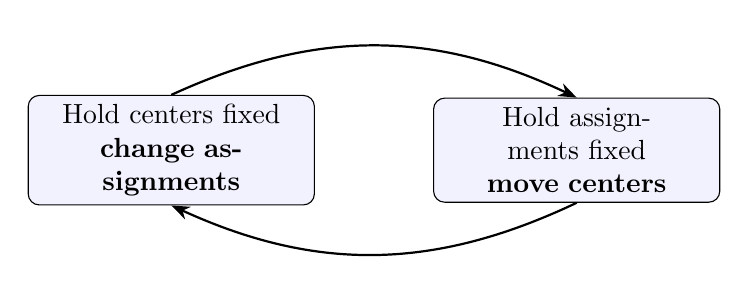
\begin{tikzpicture}[node distance=1.5cm,>=Stealth]
\node[draw,rounded corners,fill=blue!5,text width=3.4cm,align=center] (a) {Hold centers fixed\\\textbf{change assignments}};
\node[draw,rounded corners,fill=blue!5,text width=3.4cm,align=center,right=of a] (b) {Hold assignments fixed\\\textbf{move centers}};
\draw[->,thick] (a.north) to[bend left=25] (b.north);
\draw[->,thick] (b.south) to[bend left=25] (a.south);
\end{tikzpicture}
\end{center}
\ask{Why might moving a center change which points are closest to it?}
\note{Do not combine the two steps prematurely. This separation is the central learning objective of the dashboard. One full iteration includes assignment and update.}
\end{frame}

\begin{frame}{The objective: total squared distance}
\small
Let $n$ be the number of observations, $p$ the number of features, and $K$ the number of groups. Let $c_i\in\{1,\ldots,K\}$ assign point $i$ to a group.
\normalsize
\[
\min_{c_1,\ldots,c_n,\,\mm_1,\ldots,\mm_K}
J=\sum_{i=1}^n\norm{\xx_i-\mm_{c_i}}^2
=\sum_{k=1}^K\sum_{i\in C_k}\sum_{j=1}^p(x_{ij}-\mu_{kj})^2.
\]
\begin{itemize}
\item $J$ is the \textbf{within-cluster sum of squares} (WCSS), also called \textbf{inertia}.
\item Every point contributes its squared distance to its assigned center.
\item Regression SSE measured prediction errors; here SSE measures discrepancies from group representatives.
\end{itemize}
\src{ISLP, Section 12.4.1; \href{https://scikit-learn.org/stable/modules/clustering.html}{scikit-learn clustering guide}.}
\note{Do not describe this as a sum of unweighted cluster-average losses: larger groups contribute more terms. KMeans jointly optimizes assignments and centers, which makes the full problem difficult even though each conditional step is simple.}
\end{frame}

\begin{frame}{Assignment: choose the nearest center}
For fixed centers, assign point $i$ by
\[
c_i=\argmin_{k\in\{1,\ldots,K\}}\norm{\xx_i-\mm_k}^2.
\]
\begin{block}{Example}
For $\xx=(3,1)$ and centers $(1,1.5)$ and $(6,1.5)$:
\begin{align*}
d_1^2&=(3-1)^2+(1-1.5)^2=4.25,\\
d_2^2&=(3-6)^2+(1-1.5)^2=9.25.
\end{align*}
Assign the point to group 1.
\end{block}
\begin{itemize}
\item Squared and ordinary Euclidean distance give the same nearest center.
\item Resolve exact ties consistently, for example by the lowest cluster index.
\end{itemize}
\note{No square root is needed for the comparison. A point receives exactly one membership; the tie convention is needed for a proper partition.}
\end{frame}

\begin{frame}{Update: replace centers with group means}
Hold assignments fixed. For each nonempty group,
\[
\mm_k^{\text{new}}=\frac{1}{|C_k|}\sum_{i\in C_k}\xx_i.
\]
\begin{block}{Example}
If one group contains $(1,1)$, $(1,2)$, and $(3,1)$, then
\[
\mm_1^{\text{new}}=
\left(\frac{1+1+3}{3},\frac{1+2+1}{3}\right)
=\left(\frac53,\frac43\right).
\]
\end{block}
\ask{The center moves. Do the points move? Do their memberships change during this update?}
\small Points stay fixed; memberships wait until the next assignment step.
\note{The answer to both first questions about the observations is no. The center is recomputed; it is not another data point travelling through the dataset. Empty groups require an explicit handling rule; see appendix.}
\end{frame}

\begin{frame}{Why does the mean minimize squared error?}
Fix a group $C_k$ and one feature $j$. Minimize
\[
Q(\mu_{kj})=\sum_{i\in C_k}(x_{ij}-\mu_{kj})^2.
\]
\begin{align*}
\frac{\partial Q}{\partial\mu_{kj}}
&=-2\sum_{i\in C_k}(x_{ij}-\mu_{kj})\\
&=-2\sum_{i\in C_k}x_{ij}+2|C_k|\mu_{kj}=0.
\end{align*}
Therefore,
\[
\boxed{\widehat\mu_{kj}=\frac{1}{|C_k|}\sum_{i\in C_k}x_{ij}}.
\]
The second derivative is $2|C_k|>0$, so this is a minimum. Apply the result to every feature.
\note{This echoes the squared-error minimization used for OLS. The conditional update has a closed-form answer, so no gradient descent is needed to find the mean. Define every subscript before manipulating the equation.}
\end{frame}

\begin{frame}{A six-point example: first assignment}
\small
Use $K=2$ with initial centers $\mm_1=(1,1)$ and $\mm_2=(3,1)$.
\begin{columns}[T]
\column{0.49\textwidth}
\centering
\begin{tabular}{crrr}\toprule
Point & $d_1^2$ & $d_2^2$ & Group\\\midrule
A $(1,1)$ & 0 & 4 & 1\\
B $(1,2)$ & 1 & 5 & 1\\
C $(3,1)$ & 4 & 0 & 2\\
D $(6,2)$ & 26 & 10 & 2\\
E $(7,1)$ & 36 & 16 & 2\\
F $(8,2)$ & 50 & 26 & 2\\\bottomrule
\end{tabular}
\column{0.49\textwidth}
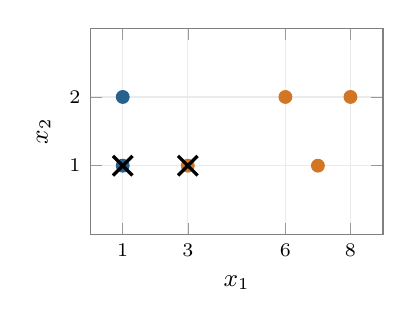
\begin{tikzpicture}
\begin{axis}[width=5.3cm,height=4.2cm,xlabel={$x_1$},ylabel={$x_2$},xmin=0,xmax=9,ymin=0,ymax=3,xtick={1,3,6,8},ytick={1,2}]
\addplot[only marks,mark=*,mark size=2.3pt,cA] coordinates {(1,1)(1,2)};
\addplot[only marks,mark=*,mark size=2.3pt,cB] coordinates {(3,1)(6,2)(7,1)(8,2)};
\addplot[only marks,mark=x,mark size=5pt,very thick,black] coordinates {(1,1)(3,1)};
\end{axis}
\end{tikzpicture}
\end{columns}
\[
J=0+1+0+10+16+26=53.
\]
\src{Illustrative points in arbitrary numerical units; not sampled weather data.}
\note{Let students check one row. This initialization is deliberately imperfect so a later point changes groups. Distinguish the data points from the black center crosses that initially overlap two points.}
\end{frame}

\begin{frame}{Move the centers, then reconsider membership}
\small
First update: $\mm_1=(1,1.5)$ and $\mm_2=(6,1.5)$.
\begin{center}
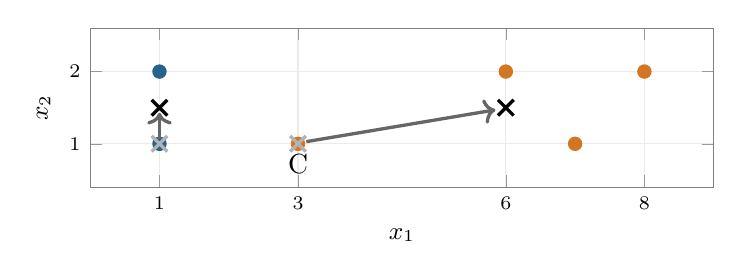
\begin{tikzpicture}
\begin{axis}[width=9.5cm,height=3.6cm,xlabel={$x_1$},ylabel={$x_2$},xmin=0,xmax=9,ymin=0.4,ymax=2.6,xtick={1,3,6,8},ytick={1,2}]
\addplot[only marks,mark=*,mark size=2.4pt,cA] coordinates {(1,1)(1,2)};
\addplot[only marks,mark=*,mark size=2.4pt,cB] coordinates {(3,1)(6,2)(7,1)(8,2)};
\addplot[only marks,mark=x,mark size=4pt,very thick,black!30] coordinates {(1,1)(3,1)};
\addplot[only marks,mark=x,mark size=4pt,very thick,black] coordinates {(1,1.5)(6,1.5)};
\draw[->,very thick,black!60] (axis cs:1,1.06)--(axis cs:1,1.43);
\draw[->,very thick,black!60] (axis cs:3.12,1.03)--(axis cs:5.85,1.47);
\node[anchor=north] at (axis cs:3,0.98) {C};
\end{axis}
\end{tikzpicture}
\end{center}
\vspace{-0.4em}
\begin{itemize}
\item Update: keep groups fixed; SSE falls from $53$ to $15.5$.
\item Reassign: C is now closer to center 1; SSE falls to $10.5$.
\item Update again: centers become $(5/3,4/3)$ and $(7,5/3)$; SSE is $6$.
\end{itemize}
\note{The arrows show actual centroid paths from the first update. Ask for C's comparison using the earlier 4.25 versus 9.25 calculation. The change in SSE is five because only C changes assignment in that step.}
\end{frame}

\begin{frame}{The objective falls and then levels off}
\begin{center}
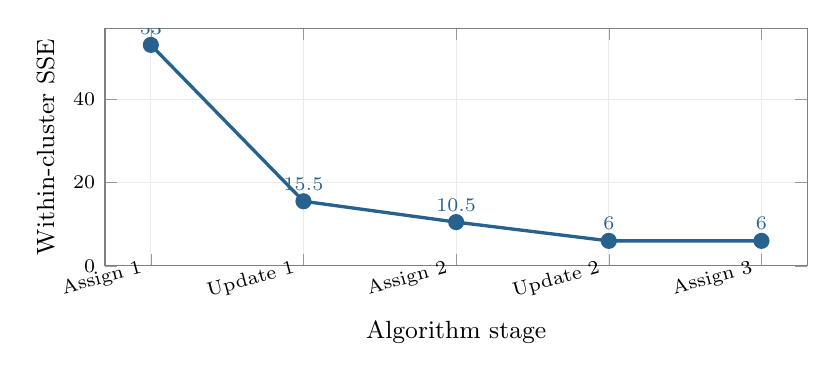
\begin{tikzpicture}
\begin{axis}[width=10.5cm,height=4.6cm,xlabel={Algorithm stage},ylabel={Within-cluster SSE},xmin=0.7,xmax=5.3,ymin=0,ymax=57,xtick={1,2,3,4,5},xticklabels={Assign 1,Update 1,Assign 2,Update 2,Assign 3},x tick label style={font=\scriptsize,rotate=15,anchor=east}]
\addplot[very thick,cA,mark=*,mark size=2.3pt,nodes near coords,point meta=y,every node near coord/.append style={font=\scriptsize,anchor=south}] coordinates {(1,53)(2,15.5)(3,10.5)(4,6)(5,6)};
\end{axis}
\end{tikzpicture}
\end{center}
\begin{block}{Converged grouping}
Group 1: A, B, C.\qquad Group 2: D, E, F.\\
Another assignment makes no changes. The objective can stay equal.
\end{block}
\note{Use the flat last segment to correct the common claim that KMeans strictly decreases the objective at every stage. The chart is exact for the illustrative six-point dataset.}
\end{frame}

\begin{frame}{Why can't an exact step increase the objective?}
\begin{enumerate}
\item \textbf{Assignment:} each point chooses its closest fixed center. Its squared-distance contribution cannot get larger.
\item \textbf{Update:} the mean minimizes squared distance for each fixed group. Each group's contribution cannot get larger.
\end{enumerate}
\[
J_{\mathrm{after\ assignment}}\leq J_{\mathrm{before}},\qquad
J_{\mathrm{after\ update}}\leq J_{\mathrm{after\ assignment}}.
\]
\begin{block}{What convergence means}
With consistent ties and valid updates, the ideal finite-data algorithm settles at a fixed grouping. Implementations may also stop at a tolerance or iteration limit.
\end{block}
\small A stable solution need not be the global minimum.
\note{The finite convergence statement refers to exact Lloyd updates, consistent tie-breaking, and a defined empty-cluster policy. Floating-point stopping and max\_iter are practical implementation conditions. Avoid saying the objective is globally convex.}
\end{frame}

\begin{frame}{Convergence does not guarantee the best grouping}
\small Same four observations, same $K=2$, two stable solutions:
\begin{columns}[T]
\column{0.49\textwidth}
\centering
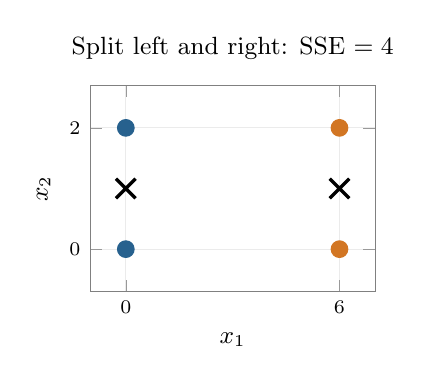
\begin{tikzpicture}
\begin{axis}[width=5.2cm,height=4.2cm,title={Split left and right: SSE $=4$},xmin=-1,xmax=7,ymin=-0.7,ymax=2.7,xtick={0,6},ytick={0,2},xlabel={$x_1$},ylabel={$x_2$}]
\addplot[only marks,mark=*,mark size=3pt,cA] coordinates {(0,0)(0,2)};
\addplot[only marks,mark=*,mark size=3pt,cB] coordinates {(6,0)(6,2)};
\addplot[only marks,mark=x,mark size=5pt,very thick,black] coordinates {(0,1)(6,1)};
\end{axis}
\end{tikzpicture}
\column{0.49\textwidth}
\centering
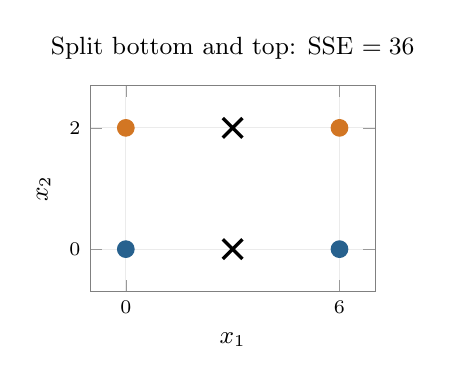
\begin{tikzpicture}
\begin{axis}[width=5.2cm,height=4.2cm,title={Split bottom and top: SSE $=36$},xmin=-1,xmax=7,ymin=-0.7,ymax=2.7,xtick={0,6},ytick={0,2},xlabel={$x_1$},ylabel={$x_2$}]
\addplot[only marks,mark=*,mark size=3pt,cA] coordinates {(0,0)(6,0)};
\addplot[only marks,mark=*,mark size=3pt,cB] coordinates {(0,2)(6,2)};
\addplot[only marks,mark=x,mark size=5pt,very thick,black] coordinates {(3,0)(3,2)};
\end{axis}
\end{tikzpicture}
\end{columns}
\ask{In the right panel, why does neither alternating step change anything?}
\src{Illustrative points; crosses are centroids. Different initializations can reach different solutions.}
\note{The top/bottom solution is a genuine fixed point: each point is nearer its own center, and each center is the mean of its two points. This concrete counterexample is easier than an abstract statement about local minima.}
\end{frame}

\begin{frame}{Better starting centers and multiple restarts}
\begin{block}{KMeans++ initialization}
Choose the first center randomly. Favor later points that are far from all chosen centers:
\[
P(\xx_i\text{ chosen next})\propto D(\xx_i)^2,
\]
where $D(\xx_i)$ is distance to its nearest chosen center.
\end{block}
\begin{itemize}
\item Run the full algorithm from multiple starts.
\item Keep the run with the lowest final inertia for the \textbf{same data, features, scaling, and $K$}.
\item Use a fixed random seed to reproduce the experiment.
\item The notebook uses 20 starts; better initialization does not guarantee a global optimum.
\end{itemize}
\src{\href{https://scikit-learn.org/stable/modules/generated/sklearn.cluster.KMeans.html}{scikit-learn KMeans API}; its implementation uses a greedy variant of KMeans++.}
\note{The equation describes the standard seeding idea. Scikit-learn tries multiple candidates at each seeding step, a detail students do not need to implement. n\_init counts full restarts; max\_iter caps iterations inside a single restart.}
\end{frame}

\begin{frame}{The weather data in two dimensions}
\begin{center}
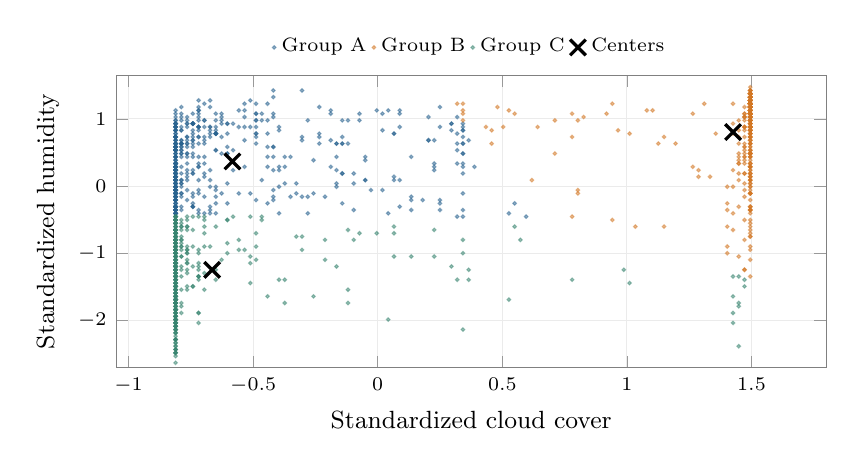
\begin{tikzpicture}
\begin{axis}[width=10.6cm,height=5.3cm,xlabel={Standardized cloud cover},ylabel={Standardized humidity},legend style={at={(0.5,1.025)},anchor=south,legend columns=4},xmin=-1.05,xmax=1.8,ymin=-2.7,ymax=1.65]
\addplot[only marks,mark=*,mark size=0.65pt,color=cA,opacity=0.48] coordinates {
(0.59547,-0.45348)
(-0.16561,0.03995)
(0.31872,0.33602)
(-0.48849,0.63208)
(0.34178,0.73076)
(-0.81137,0.92814)
(-0.46542,0.97748)
(-0.18867,1.12551)
(-0.53461,1.22420)
(-0.48849,1.22420)
(-0.48849,1.07617)
(-0.62687,0.48405)
(-0.48849,0.87879)
(-0.32705,0.03995)
(-0.81137,0.53339)
(-0.71912,0.43470)
(0.34178,0.63208)
(-0.51155,1.27354)
(-0.41930,1.42157)
(-0.14254,0.18799)
(-0.16561,-0.00939)
(-0.30398,-0.15742)
(-0.46542,0.08930)
(-0.05029,0.08930)
(-0.64993,0.82945)
(-0.71912,1.27354)
(-0.81137,1.07617)
(-0.78831,1.02683)
(-0.81137,0.73076)
(-0.81137,0.73076)
(-0.81137,0.43470)
(-0.81137,0.58273)
(-0.81137,0.48405)
(-0.81137,0.18799)
(-0.81137,0.33602)
(-0.81137,0.53339)
(-0.71912,1.12551)
(-0.64993,0.78011)
(-0.71912,0.28667)
(-0.67299,-0.30545)
(-0.81137,-0.40414)
(-0.81137,-0.35479)
(-0.81137,-0.10808)
(-0.81137,0.38536)
(-0.81137,0.58273)
(-0.81137,0.73076)
(-0.74218,0.92814)
(-0.74218,0.92814)
(-0.69605,0.87879)
(-0.74218,0.92814)
(-0.74218,0.92814)
(-0.67299,1.27354)
(-0.81137,0.33602)
(-0.74218,-0.10808)
(-0.81137,-0.20676)
(-0.81137,0.13864)
(-0.81137,0.58273)
(-0.81137,0.73076)
(-0.81137,0.63208)
(-0.81137,0.58273)
(0.34178,0.82945)
(0.29565,0.92814)
(-0.78831,0.82945)
(-0.71912,0.87879)
(-0.76524,0.92814)
(-0.78831,1.07617)
(-0.71912,1.17486)
(-0.71912,0.87879)
(-0.71912,0.28667)
(-0.78831,-0.30545)
(-0.81137,-0.05873)
(-0.81137,0.23733)
(-0.81137,0.78011)
(-0.07335,1.07617)
(-0.81137,0.92814)
(-0.81137,0.82945)
(-0.81137,0.92814)
(-0.81137,0.87879)
(-0.71912,1.07617)
(-0.81137,0.87879)
(-0.81137,0.53339)
(-0.81137,0.08930)
(-0.35011,-0.15742)
(0.24953,-0.25611)
(0.08809,0.87879)
(-0.14254,0.63208)
(0.31872,0.53339)
(-0.76524,0.48405)
(-0.44236,0.43470)
(-0.74218,0.73076)
(-0.18867,0.68142)
(-0.14254,0.63208)
(-0.07335,0.97748)
(0.31872,0.63208)
(-0.74218,0.18799)
(0.13421,-0.15742)
(-0.37317,0.03995)
(0.34178,-0.10808)
(-0.44236,-0.25611)
(-0.39624,0.23733)
(-0.05029,0.08930)
(-0.44236,0.28667)
(-0.48849,0.78011)
(-0.62687,1.02683)
(0.24953,0.87879)
(-0.48849,1.07617)
(0.06502,0.78011)
(-0.39624,0.28667)
(-0.32705,-0.10808)
(-0.25786,-0.10808)
(-0.14254,-0.25611)
(-0.09642,-0.35479)
(-0.81137,-0.35479)
(-0.81137,-0.10808)
(-0.71912,0.33602)
(-0.78831,0.48405)
(-0.81137,0.33602)
(-0.81137,0.68142)
(-0.51155,0.87879)
(0.13421,0.43470)
(-0.09642,0.18799)
(-0.28092,-0.15742)
(0.52628,-0.40414)
(0.08809,-0.30545)
(-0.69605,-0.15742)
(-0.67299,0.23733)
(-0.62687,0.97748)
(-0.39624,0.82945)
(-0.78831,0.87879)
(-0.81137,0.87879)
(-0.71912,1.02683)
(-0.64993,1.07617)
(-0.81137,1.02683)
(-0.74218,1.07617)
(-0.23479,1.17486)
(-0.78831,1.17486)
(0.34178,0.87879)
(-0.23479,0.78011)
(0.20340,0.68142)
(-0.11948,0.63208)
(-0.05029,0.38536)
(0.34178,0.48405)
(-0.60380,0.48405)
(0.34178,0.28667)
(-0.09642,0.03995)
(-0.64993,-0.00939)
(-0.41930,-0.15742)
(-0.76524,-0.20676)
(-0.76524,0.33602)
(-0.74218,0.58273)
(-0.81137,0.82945)
(-0.41930,1.07617)
(-0.69605,0.97748)
(-0.58074,0.92814)
(0.20340,1.02683)
(-0.64993,0.78011)
(-0.78831,0.58273)
(-0.81137,0.33602)
(-0.81137,0.23733)
(-0.81137,0.33602)
(-0.81137,0.13864)
(-0.69605,0.13864)
(-0.71912,-0.10808)
(-0.48849,-0.20676)
(0.08809,0.08930)
(0.06502,0.13864)
(-0.74218,0.23733)
(-0.64993,-0.05873)
(-0.21173,-0.15742)
(0.34178,-0.45348)
(0.31872,-0.45348)
(0.24953,-0.35479)
(-0.28092,-0.40414)
(-0.74218,-0.15742)
(-0.76524,0.08930)
(-0.81137,0.43470)
(-0.16561,0.23733)
(-0.39624,-0.00939)
(-0.81137,0.33602)
(0.34178,0.33602)
(0.34178,0.48405)
(-0.16561,0.63208)
(0.06502,0.08930)
(0.34178,-0.35479)
(-0.39624,-0.40414)
(0.22647,0.68142)
(-0.30398,0.73076)
(-0.71912,0.87879)
(-0.64993,0.78011)
(-0.48849,0.73076)
(-0.53461,0.28667)
(0.01890,-0.05873)
(0.13421,-0.20676)
(-0.41930,-0.20676)
(-0.67299,-0.40414)
(-0.71912,-0.35479)
(-0.81137,-0.00939)
(-0.81137,0.18799)
(-0.81137,0.53339)
(-0.81137,0.68142)
(-0.71912,0.97748)
(-0.60380,0.92814)
(0.04196,1.12551)
(0.29565,0.92814)
(-0.11948,0.97748)
(-0.64993,0.78011)
(-0.71912,0.73076)
(-0.71912,0.87879)
(-0.76524,0.92814)
(-0.81137,1.12551)
(-0.76524,0.73076)
(-0.76524,0.13864)
(-0.74218,-0.30545)
(-0.62687,-0.10808)
(-0.48849,0.78011)
(0.36484,0.68142)
(-0.81137,0.63208)
(-0.78831,0.63208)
(-0.76524,0.87879)
(-0.81137,0.53339)
(-0.35011,0.43470)
(-0.14254,0.97748)
(-0.81137,0.87879)
(-0.81137,0.73076)
(-0.81137,0.92814)
(-0.48849,0.97748)
(-0.44236,0.58273)
(-0.74218,-0.30545)
(-0.81137,-0.35479)
(-0.81137,-0.10808)
(-0.81137,-0.00939)
(-0.81137,0.13864)
(-0.81137,0.08930)
(-0.81137,-0.00939)
(-0.78831,-0.15742)
(-0.78831,0.28667)
(-0.81137,0.33602)
(-0.81137,0.63208)
(-0.81137,0.53339)
(-0.81137,0.03995)
(-0.23479,0.73076)
(-0.18867,1.07617)
(0.34178,0.82945)
(-0.14254,0.18799)
(-0.81137,-0.20676)
(-0.81137,-0.30545)
(-0.81137,-0.00939)
(-0.81137,0.53339)
(-0.81137,0.23733)
(-0.81137,0.08930)
(-0.81137,0.28667)
(-0.81137,0.68142)
(-0.78831,0.82945)
(-0.69605,1.22420)
(-0.81137,0.43470)
(-0.81137,-0.30545)
(-0.78831,0.43470)
(-0.53461,0.87879)
(-0.60380,0.92814)
(0.31872,1.02683)
(-0.76524,0.97748)
(-0.81137,0.97748)
(-0.81137,0.82945)
(-0.78831,0.68142)
(-0.76524,-0.05873)
(-0.81137,-0.05873)
(-0.81137,0.28667)
(-0.81137,0.28667)
(-0.81137,0.18799)
(-0.81137,0.23733)
(-0.81137,-0.25611)
(-0.81137,-0.20676)
(-0.81137,-0.15742)
(-0.81137,-0.30545)
(-0.81137,-0.35479)
(-0.71912,-0.40414)
(-0.81137,-0.30545)
(-0.81137,-0.15742)
(0.13421,-0.35479)
(0.24953,1.17486)
(-0.81137,0.92814)
(-0.81137,0.87879)
(-0.78831,0.58273)
(-0.81137,0.53339)
(-0.81137,0.82945)
(-0.81137,0.28667)
(-0.81137,-0.30545)
(-0.67299,-0.00939)
(-0.81137,-0.15742)
(-0.81137,0.33602)
(-0.81137,0.18799)
(-0.76524,0.23733)
(-0.67299,0.73076)
(-0.64993,0.97748)
(-0.74218,0.82945)
(-0.81137,0.33602)
(-0.81137,-0.00939)
(-0.81137,-0.40414)
(-0.81137,0.18799)
(-0.81137,0.58273)
(-0.81137,0.18799)
(-0.81137,-0.25611)
(-0.81137,-0.00939)
(-0.81137,0.33602)
(-0.81137,0.13864)
(-0.81137,0.03995)
(-0.81137,-0.05873)
(-0.81137,-0.05873)
(-0.81137,-0.30545)
(-0.81137,-0.40414)
(-0.81137,-0.40414)
(-0.81137,-0.30545)
(-0.81137,-0.15742)
(-0.81137,-0.35479)
(-0.81137,-0.30545)
(-0.81137,-0.35479)
(-0.74218,-0.30545)
(0.54935,-0.25611)
(-0.53461,1.02683)
(-0.81137,0.97748)
(0.31872,0.78011)
(-0.39624,0.87879)
(-0.62687,0.92814)
(-0.69605,0.68142)
(-0.69605,0.43470)
(-0.81137,0.08930)
(-0.81137,-0.15742)
(-0.78831,-0.35479)
(-0.60380,-0.25611)
(-0.02723,-0.05873)
(0.18034,-0.20676)
(-0.81137,-0.20676)
(-0.81137,-0.10808)
(-0.81137,-0.35479)
(-0.81137,-0.30545)
(-0.81137,-0.00939)
(-0.81137,0.23733)
(-0.81137,-0.40414)
(-0.81137,-0.20676)
(-0.81137,0.28667)
(-0.81137,0.28667)
(-0.81137,0.23733)
(-0.81137,-0.10808)
(-0.81137,-0.40414)
(-0.81137,0.13864)
(-0.81137,0.53339)
(-0.74218,0.92814)
(-0.41930,1.02683)
(-0.25786,0.38536)
(-0.78831,0.53339)
(-0.76524,0.73076)
(-0.60380,0.58273)
(-0.74218,0.63208)
(-0.76524,0.63208)
(-0.81137,0.63208)
(-0.81137,-0.35479)
(-0.81137,0.03995)
(-0.81137,0.03995)
(-0.81137,-0.30545)
(-0.81137,-0.30545)
(-0.81137,-0.30545)
(-0.81137,-0.10808)
(-0.81137,-0.10808)
(-0.81137,0.13864)
(-0.81137,-0.05873)
(-0.81137,-0.20676)
(-0.81137,-0.05873)
(-0.81137,-0.05873)
(-0.81137,-0.10808)
(-0.78831,0.08930)
(-0.81137,-0.00939)
(-0.81137,0.08930)
(-0.81137,0.03995)
(-0.81137,0.08930)
(-0.81137,-0.05873)
(-0.78831,0.53339)
(-0.81137,-0.00939)
(-0.81137,-0.15742)
(-0.81137,-0.05873)
(-0.81137,-0.10808)
(-0.78831,0.03995)
(-0.78831,0.08930)
(-0.78831,-0.00939)
(-0.81137,-0.10808)
(-0.78831,-0.10808)
(-0.81137,-0.15742)
(-0.81137,0.08930)
(-0.81137,0.08930)
(-0.81137,-0.35479)
(-0.81137,0.18799)
(-0.78831,0.63208)
(-0.81137,0.63208)
(-0.81137,0.82945)
(-0.71912,1.12551)
(-0.81137,0.73076)
(-0.71912,0.82945)
(-0.78831,0.68142)
(-0.71912,0.73076)
(-0.69605,0.73076)
(-0.60380,0.78011)
(-0.67299,0.82945)
(-0.41930,1.32289)
(-0.14254,0.73076)
(-0.71912,-0.05873)
(-0.64993,-0.15742)
(-0.71912,0.08930)
(-0.78831,0.63208)
(-0.78831,0.63208)
(-0.74218,0.68142)
(-0.67299,0.87879)
(-0.64993,0.87879)
(-0.74218,0.92814)
(0.22647,0.23733)
(-0.69605,-0.40414)
(-0.81137,-0.25611)
(-0.81137,0.28667)
(-0.74218,0.18799)
(0.22647,0.28667)
(-0.60380,0.48405)
(-0.81137,0.23733)
(-0.81137,0.33602)
(-0.81137,0.28667)
(-0.81137,0.18799)
(-0.81137,0.33602)
(-0.81137,0.13864)
(-0.81137,0.13864)
(-0.69605,0.18799)
(-0.81137,0.68142)
(-0.81137,0.87879)
(-0.81137,0.73076)
(-0.81137,0.28667)
(-0.81137,-0.15742)
(-0.81137,-0.00939)
(-0.81137,0.43470)
(-0.78831,0.48405)
(-0.81137,-0.30545)
(-0.81137,-0.35479)
(-0.81137,-0.10808)
(-0.81137,0.03995)
(-0.76524,0.18799)
(-0.81137,0.13864)
(-0.81137,0.08930)
(-0.81137,-0.35479)
(-0.67299,0.78011)
(0.29565,0.82945)
(0.06502,0.78011)
(0.01890,0.82945)
(-0.64993,0.78011)
(-0.81137,0.48405)
(-0.69605,0.63208)
(-0.23479,0.63208)
(-0.05029,0.43470)
(0.34178,0.18799)
(0.22647,0.33602)
(-0.76524,0.68142)
(0.20340,0.68142)
(0.34178,0.92814)
(-0.00416,1.12551)
(-0.62687,1.07617)
(0.08809,1.12551)
(0.01890,1.07617)
(-0.30398,1.42157)
(-0.67299,0.87879)
(-0.78831,0.18799)
(-0.67299,-0.35479)
(-0.81137,-0.35479)
(-0.81137,0.18799)
(-0.81137,0.38536)
(-0.81137,0.33602)
(-0.81137,0.23733)
(-0.81137,0.33602)
(-0.81137,0.08930)
(-0.81137,-0.30545)
(-0.81137,-0.00939)
(-0.81137,-0.05873)
(-0.41930,-0.05873)
(-0.81137,-0.20676)
(-0.60380,0.03995)
(-0.81137,0.48405)
(-0.78831,-0.10808)
(0.24953,-0.20676)
(-0.41930,0.43470)
(-0.74218,0.48405)
(-0.76524,0.43470)
(-0.69605,0.33602)
(-0.16561,0.43470)
(-0.16561,0.63208)
(-0.58074,0.23733)
(-0.76524,0.48405)
(-0.81137,0.58273)
(-0.81137,0.03995)
(-0.74218,-0.25611)
(-0.51155,-0.10808)
(-0.41930,0.23733)
(-0.41930,0.58273)
(-0.62687,0.73076)
(0.04196,-0.40414)
(-0.81137,-0.00939)
(-0.81137,0.08930)
(-0.81137,0.43470)
(-0.76524,0.63208)
(-0.37317,0.28667)
(-0.81137,0.73076)
(-0.81137,0.33602)
(-0.81137,0.23733)
(-0.81137,-0.00939)
(-0.81137,0.53339)
(0.34178,0.63208)
(-0.81137,0.78011)
(-0.64993,0.53339)
(-0.78831,0.03995)
(-0.64993,-0.40414)
(-0.81137,-0.05873)
(-0.81137,0.18799)
(-0.81137,0.38536)
(-0.81137,0.58273)
(-0.81137,0.63208)
(-0.81137,0.58273)
(-0.81137,0.53339)
(-0.76524,0.58273)
(-0.78831,0.97748)
(-0.53461,1.12551)
(-0.55768,1.12551)
(-0.76524,1.02683)
(-0.69605,0.97748)
(-0.67299,1.17486)
(-0.58074,0.53339)
(-0.55768,-0.10808)
(-0.74218,0.43470)
(-0.37317,0.43470)
(0.08809,1.07617)
(-0.48849,0.97748)
(-0.44236,0.78011)
(-0.74218,0.78011)
(-0.74218,0.68142)
(-0.78831,0.63208)
(-0.44236,1.22420)
(-0.28092,0.97748)
(-0.41930,0.58273)
(-0.67299,0.08930)
(-0.81137,0.13864)
(-0.81137,-0.00939)
(-0.64993,0.53339)
(-0.44236,0.97748)
(-0.46542,1.07617)
(-0.30398,0.68142)
(-0.71912,0.63208)
(-0.53461,0.68142)
(-0.55768,0.87879)
(0.38791,0.28667)
(-0.18867,0.28667)
(-0.64993,-0.25611)
(-0.81137,-0.30545)
(-0.81137,-0.40414)
(-0.81137,-0.05873)
(-0.81137,-0.35479)
(-0.81137,-0.20676)
(-0.81137,-0.30545)
};
\addlegendentry{Group A}
\addplot[only marks,mark=*,mark size=0.65pt,color=cB,opacity=0.48] coordinates {
(1.49493,1.07617)
(1.49493,1.07617)
(1.49493,1.07617)
(1.49493,0.63208)
(1.49493,0.28667)
(1.49493,0.13864)
(1.49493,0.23733)
(1.47187,0.43470)
(1.47187,0.58273)
(1.49493,1.02683)
(1.49493,1.22420)
(1.49493,1.32289)
(1.49493,1.22420)
(1.49493,1.17486)
(1.49493,1.32289)
(1.49493,1.12551)
(1.49493,1.02683)
(1.49493,1.07617)
(1.49493,1.27354)
(1.49493,1.32289)
(1.49493,1.17486)
(1.49493,1.07617)
(1.49493,0.97748)
(1.49493,0.87879)
(1.49493,1.22420)
(1.49493,1.17486)
(1.49493,0.78011)
(1.49493,0.68142)
(0.50322,0.87879)
(1.49493,0.97748)
(1.49493,1.12551)
(1.49493,1.17486)
(1.49493,1.27354)
(1.49493,1.12551)
(1.49493,1.12551)
(1.49493,1.17486)
(1.49493,1.22420)
(1.49493,1.27354)
(1.49493,1.32289)
(1.49493,1.32289)
(1.49493,1.37223)
(1.49493,1.32289)
(1.49493,1.27354)
(1.49493,1.07617)
(1.49493,0.48405)
(1.49493,-0.65086)
(0.54935,1.07617)
(1.49493,1.07617)
(1.49493,1.12551)
(1.49493,1.07617)
(1.49493,1.22420)
(1.31043,1.22420)
(1.49493,1.22420)
(1.49493,1.17486)
(1.47187,0.53339)
(0.34178,0.97748)
(1.49493,-0.10808)
(1.49493,0.58273)
(0.31872,1.22420)
(0.48016,1.17486)
(1.49493,0.97748)
(1.49493,1.02683)
(1.49493,0.63208)
(1.49493,0.78011)
(1.49493,0.48405)
(1.49493,0.28667)
(1.49493,0.18799)
(1.49493,0.48405)
(1.49493,0.48405)
(1.49493,0.82945)
(1.49493,0.68142)
(1.49493,0.73076)
(1.49493,0.23733)
(1.49493,0.28667)
(1.49493,1.07617)
(0.71079,0.97748)
(1.03367,-0.60151)
(1.49493,-0.60151)
(0.80304,-0.10808)
(1.14899,0.73076)
(0.64160,0.87879)
(0.77998,1.07617)
(1.49493,0.97748)
(1.49493,0.82945)
(1.49493,0.97748)
(1.49493,0.73076)
(1.49493,0.78011)
(1.49493,0.63208)
(1.49493,0.68142)
(1.49493,0.78011)
(1.49493,0.58273)
(1.49493,0.87879)
(1.49493,1.12551)
(1.49493,1.12551)
(1.49493,1.07617)
(1.49493,1.07617)
(1.49493,1.27354)
(1.49493,1.17486)
(1.49493,1.27354)
(1.49493,1.27354)
(1.49493,1.27354)
(1.49493,1.22420)
(1.49493,1.27354)
(1.49493,1.22420)
(1.49493,1.12551)
(1.49493,1.27354)
(1.49493,1.17486)
(1.49493,1.27354)
(1.49493,0.97748)
(1.49493,1.22420)
(1.49493,1.02683)
(1.49493,0.92814)
(1.49493,1.32289)
(1.49493,1.12551)
(1.49493,1.17486)
(1.49493,1.27354)
(1.49493,1.32289)
(1.49493,1.27354)
(1.49493,1.22420)
(1.49493,1.22420)
(1.49493,1.22420)
(1.49493,1.22420)
(1.49493,1.27354)
(1.49493,1.27354)
(1.49493,1.22420)
(1.49493,1.12551)
(1.49493,1.07617)
(1.49493,1.12551)
(1.49493,1.12551)
(1.49493,1.07617)
(1.49493,1.37223)
(1.49493,1.22420)
(1.49493,1.22420)
(1.49493,1.22420)
(1.49493,1.22420)
(1.49493,1.27354)
(1.49493,1.32289)
(1.49493,1.27354)
(1.49493,1.12551)
(1.49493,1.07617)
(1.49493,1.02683)
(1.49493,1.12551)
(1.49493,0.97748)
(1.49493,0.53339)
(1.49493,0.43470)
(1.49493,0.48405)
(1.49493,0.38536)
(1.49493,0.43470)
(1.49493,-0.35479)
(1.49493,-0.35479)
(1.49493,-0.50282)
(1.49493,1.07617)
(1.49493,-0.55217)
(1.49493,-0.30545)
(1.42574,0.92814)
(1.49493,0.92814)
(0.96448,0.82945)
(1.12592,0.63208)
(1.49493,-1.09495)
(1.49493,-0.89757)
(1.47187,-0.79889)
(1.49493,-0.74954)
(1.49493,-0.10808)
(1.49493,0.33602)
(1.49493,0.48405)
(1.49493,0.08930)
(1.49493,0.03995)
(1.49493,0.18799)
(1.49493,0.97748)
(1.01061,0.78011)
(0.34178,1.07617)
(1.49493,-0.10808)
(1.49493,-0.10808)
(1.40268,-0.00939)
(0.34178,1.22420)
(0.71079,0.48405)
(1.49493,-0.00939)
(1.49493,-0.05873)
(0.82610,1.02683)
(1.49493,0.97748)
(1.49493,0.73076)
(1.49493,0.18799)
(1.49493,0.48405)
(1.49493,0.87879)
(1.49493,1.22420)
(1.49493,1.17486)
(1.49493,1.22420)
(1.49493,1.27354)
(1.49493,1.27354)
(1.49493,1.37223)
(1.49493,1.22420)
(1.47187,1.17486)
(1.47187,1.07617)
(1.49493,1.07617)
(1.49493,1.22420)
(1.49493,1.17486)
(1.49493,1.17486)
(1.49493,1.32289)
(1.49493,1.32289)
(1.49493,1.32289)
(1.49493,1.32289)
(1.49493,1.27354)
(1.49493,1.37223)
(1.49493,1.27354)
(1.49493,1.37223)
(1.49493,1.42157)
(1.49493,1.32289)
(1.49493,1.37223)
(1.49493,1.37223)
(1.49493,1.37223)
(1.49493,1.32289)
(1.49493,1.22420)
(1.49493,1.42157)
(1.49493,1.37223)
(1.49493,1.37223)
(1.49493,1.17486)
(1.49493,1.07617)
(1.49493,0.87879)
(1.49493,0.92814)
(1.49493,0.87879)
(1.49493,0.87879)
(1.49493,0.82945)
(1.49493,1.02683)
(1.49493,1.12551)
(1.49493,1.17486)
(1.49493,1.17486)
(1.42574,1.22420)
(1.49493,1.17486)
(1.49493,1.32289)
(1.49493,1.32289)
(1.49493,1.22420)
(1.49493,1.37223)
(1.49493,1.32289)
(1.49493,1.22420)
(1.49493,1.42157)
(1.49493,1.17486)
(1.47187,1.07617)
(0.91836,1.07617)
(0.52628,1.12551)
(1.07980,1.12551)
(1.49493,1.12551)
(1.49493,1.17486)
(1.40268,-0.60151)
(1.40268,-0.89757)
(1.40268,-0.99626)
(1.40268,-0.35479)
(1.40268,-0.25611)
(1.42574,-0.40414)
(1.42574,-0.00939)
(1.28736,0.23733)
(1.49493,0.43470)
(1.44880,0.38536)
(1.42574,0.78011)
(1.42574,-0.65086)
(1.44880,-1.04560)
(1.44880,-0.30545)
(1.44880,0.18799)
(1.44880,0.08930)
(1.44880,0.63208)
(1.44880,0.43470)
(1.47187,0.87879)
(1.44880,0.97748)
(0.45710,0.82945)
(1.44880,0.73076)
(1.44880,0.82945)
(1.49493,1.07617)
(1.49493,1.22420)
(1.47187,1.02683)
(1.47187,1.02683)
(1.47187,0.87879)
(1.47187,0.73076)
(1.47187,0.38536)
(1.47187,0.33602)
(1.47187,-0.15742)
(1.14899,-0.60151)
(1.49493,-0.30545)
(1.49493,-0.94692)
(1.49493,-0.10808)
(1.49493,0.13864)
(1.49493,0.33602)
(1.49493,0.08930)
(1.49493,0.13864)
(1.49493,0.08930)
(1.49493,0.73076)
(1.49493,1.07617)
(1.49493,1.02683)
(1.49493,1.07617)
(1.49493,1.22420)
(1.49493,1.22420)
(1.49493,1.27354)
(1.49493,1.17486)
(1.49493,1.17486)
(1.49493,1.27354)
(1.49493,1.17486)
(1.49493,1.32289)
(1.49493,1.27354)
(1.49493,1.32289)
(1.49493,1.27354)
(1.49493,1.32289)
(1.49493,1.17486)
(1.49493,1.12551)
(1.49493,1.22420)
(1.49493,1.22420)
(1.49493,1.17486)
(1.49493,1.22420)
(1.49493,1.32289)
(1.49493,1.37223)
(1.49493,1.37223)
(1.49493,1.32289)
(1.49493,1.22420)
(1.49493,0.82945)
(1.49493,1.12551)
(1.49493,1.17486)
(1.47187,0.18799)
(1.49493,0.87879)
(1.49493,0.87879)
(1.49493,0.87879)
(1.10286,1.12551)
(1.49493,0.92814)
(1.49493,1.02683)
(1.49493,0.87879)
(1.49493,1.12551)
(1.49493,1.27354)
(1.49493,1.07617)
(1.49493,0.97748)
(1.49493,1.12551)
(1.49493,0.82945)
(1.49493,0.87879)
(1.49493,0.97748)
(1.49493,1.07617)
(1.49493,1.12551)
(1.49493,1.12551)
(1.49493,1.22420)
(1.49493,1.22420)
(1.49493,1.22420)
(1.49493,1.27354)
(1.49493,1.22420)
(1.49493,1.22420)
(1.49493,1.27354)
(1.49493,1.37223)
(1.49493,1.17486)
(1.49493,1.27354)
(1.49493,1.32289)
(1.49493,1.22420)
(1.49493,1.07617)
(1.47187,-0.50282)
(1.47187,-0.05873)
(1.49493,-0.20676)
(1.49493,-0.35479)
(1.49493,-0.35479)
(1.49493,-0.30545)
(1.49493,0.03995)
(1.49493,0.28667)
(1.49493,0.97748)
(1.49493,0.78011)
(1.49493,0.82945)
(1.44880,0.33602)
(1.35655,0.78011)
(1.47187,0.43470)
(1.44880,0.48405)
(1.49493,-0.70020)
(0.77998,0.73076)
(1.49493,-0.74954)
(1.49493,-1.34166)
(1.49493,1.02683)
(1.49493,1.32289)
(1.49493,1.22420)
(1.49493,1.42157)
(1.49493,1.32289)
(1.49493,1.22420)
(1.49493,0.92814)
(1.49493,1.27354)
(0.34178,1.12551)
(1.49493,1.22420)
(1.49493,1.47092)
(1.49493,1.22420)
(0.43403,0.87879)
(1.47187,0.03995)
(1.47187,0.18799)
(1.33349,0.13864)
(1.49493,0.08930)
(1.26430,0.28667)
(1.49493,1.27354)
(1.49493,1.02683)
(1.49493,0.97748)
(1.49493,1.17486)
(1.49493,1.32289)
(1.49493,1.32289)
(1.47187,-1.24298)
(1.47187,-1.24298)
(0.77998,-0.45348)
(1.28736,0.13864)
(1.44880,0.33602)
(1.47187,0.48405)
(0.94142,-0.50282)
(1.47187,1.02683)
(1.47187,0.82945)
(1.47187,0.97748)
(1.47187,0.58273)
(1.47187,0.87879)
(1.19511,0.63208)
(1.47187,0.63208)
(0.80304,-0.05873)
(0.61854,0.08930)
(0.45710,0.63208)
(0.80304,0.97748)
(1.49493,0.87879)
(1.49493,0.97748)
(1.49493,1.12551)
(1.49493,0.97748)
(1.49493,1.12551)
(1.49493,1.07617)
(1.49493,0.82945)
(1.49493,0.97748)
(1.49493,0.92814)
(1.49493,0.78011)
(1.49493,0.43470)
(1.49493,0.28667)
(1.49493,0.33602)
(1.49493,0.53339)
(1.49493,0.53339)
(1.49493,0.63208)
(1.49493,0.73076)
(1.49493,0.92814)
(1.49493,0.92814)
(1.49493,1.02683)
(1.49493,1.32289)
(0.94142,1.22420)
(1.49493,1.22420)
(1.49493,1.22420)
(1.49493,1.27354)
(1.26430,1.07617)
(1.49493,-0.40414)
(1.49493,-0.00939)
(1.49493,-0.10808)
(1.42574,0.23733)
};
\addlegendentry{Group B}
\addplot[only marks,mark=*,mark size=0.65pt,color=cC,opacity=0.48] coordinates {
(-0.46542,-0.45348)
(-0.60380,-0.50282)
(-0.60380,-0.50282)
(0.06502,-0.60151)
(-0.53461,-0.94692)
(-0.21173,-1.09495)
(-0.64993,-1.24298)
(-0.78831,-1.19363)
(-0.81137,-1.19363)
(-0.81137,-0.65086)
(-0.76524,-0.50282)
(-0.78831,-0.89757)
(-0.71912,-1.14429)
(-0.74218,-1.19363)
(-0.69605,-1.29232)
(-0.71912,-1.34166)
(-0.76524,-1.29232)
(-0.81137,-1.24298)
(-0.81137,-0.99626)
(-0.81137,-0.60151)
(-0.81137,-0.65086)
(-0.81137,-0.70020)
(-0.78831,-0.79889)
(-0.81137,-0.74954)
(-0.81137,-0.74954)
(-0.81137,-0.65086)
(-0.81137,-0.79889)
(-0.81137,-0.50282)
(-0.81137,-0.50282)
(0.22647,-0.65086)
(0.06502,-0.70020)
(-0.81137,-0.94692)
(-0.76524,-1.14429)
(-0.58074,-0.45348)
(-0.69605,-0.45348)
(-0.46542,-0.50282)
(-0.51155,-0.45348)
(-0.81137,-0.94692)
(-0.81137,-1.63773)
(-0.81137,-1.83510)
(-0.81137,-1.83510)
(-0.81137,-2.03247)
(-0.81137,-2.37788)
(-0.81137,-2.37788)
(1.44880,-2.37788)
(-0.81137,-2.32854)
(-0.81137,-2.18050)
(-0.81137,-2.03247)
(0.31872,-1.39101)
(-0.81137,-0.94692)
(-0.81137,-0.94692)
(-0.81137,-1.14429)
(-0.81137,-0.99626)
(-0.81137,-1.04560)
(-0.81137,-0.89757)
(-0.81137,-0.65086)
(-0.81137,-0.65086)
(-0.81137,-0.65086)
(-0.81137,-0.70020)
(-0.81137,-0.84823)
(-0.81137,-1.14429)
(-0.81137,-1.48970)
(-0.81137,-1.58838)
(-0.81137,-1.53904)
(-0.81137,-1.63773)
(-0.81137,-1.93379)
(-0.71912,-2.03247)
(-0.78831,-1.88444)
(-0.81137,-2.08182)
(-0.81137,-2.13116)
(-0.81137,-2.13116)
(-0.32705,-0.74954)
(-0.78831,-0.79889)
(0.22647,-1.04560)
(0.77998,-1.39101)
(0.52628,-1.68707)
(1.42574,-1.34166)
(0.34178,-0.79889)
(-0.64993,-0.60151)
(-0.11948,-0.65086)
(-0.07335,-0.70020)
(0.34178,-0.99626)
(-0.30398,-0.94692)
(-0.60380,-0.99626)
(0.54935,-0.60151)
(-0.21173,-0.79889)
(-0.71912,-1.19363)
(0.36484,-1.24298)
(-0.71912,-1.34166)
(-0.39624,-1.39101)
(0.06502,-1.04560)
(-0.81137,-0.79889)
(-0.81137,-1.19363)
(-0.81137,-1.53904)
(-0.81137,-1.68707)
(-0.81137,-1.83510)
(-0.81137,-2.08182)
(-0.81137,-1.98313)
(-0.71912,-1.88444)
(-0.81137,-1.14429)
(-0.81137,-0.65086)
(-0.81137,-0.45348)
(-0.55768,-0.94692)
(-0.81137,-1.14429)
(-0.81137,-1.24298)
(-0.81137,-1.24298)
(-0.78831,-1.53904)
(-0.51155,-1.44035)
(-0.11948,-1.53904)
(0.36484,-1.39101)
(-0.16561,-1.19363)
(-0.62687,-1.09495)
(-0.81137,-0.79889)
(-0.78831,-1.04560)
(-0.76524,-1.48970)
(-0.74218,-1.48970)
(-0.78831,-1.73641)
(-0.81137,-1.78576)
(-0.81137,-1.78576)
(-0.81137,-0.94692)
(-0.81137,-0.89757)
(-0.81137,-0.50282)
(-0.81137,-0.65086)
(-0.81137,-0.84823)
(-0.81137,-1.24298)
(-0.81137,-1.44035)
(-0.81137,-1.58838)
(-0.81137,-1.73641)
(-0.81137,-1.68707)
(-0.81137,-1.73641)
(-0.81137,-1.73641)
(-0.81137,-1.53904)
(-0.81137,-0.79889)
(-0.78831,-0.55217)
(-0.76524,-0.94692)
(-0.76524,-0.94692)
(-0.76524,-0.99626)
(-0.81137,-1.29232)
(-0.81137,-1.44035)
(-0.81137,-1.24298)
(-0.81137,-0.55217)
(-0.81137,-0.70020)
(-0.81137,-0.94692)
(-0.81137,-1.19363)
(-0.81137,-1.34166)
(-0.81137,-1.53904)
(-0.78831,-1.78576)
(-0.81137,-1.73641)
(-0.81137,-1.88444)
(-0.71912,-1.88444)
(-0.81137,-1.98313)
(-0.81137,-1.48970)
(-0.81137,-1.14429)
(-0.81137,-0.65086)
(-0.81137,-0.89757)
(0.98754,-1.24298)
(1.42574,-1.63773)
(1.42574,-1.88444)
(1.42574,-2.03247)
(1.44880,-1.78576)
(1.44880,-1.73641)
(1.44880,-1.34166)
(-0.81137,-0.50282)
(-0.81137,-0.65086)
(-0.81137,-0.74954)
(-0.78831,-0.74954)
(-0.69605,-0.89757)
(-0.81137,-0.79889)
(-0.78831,-0.50282)
(-0.81137,-0.50282)
(-0.81137,-0.99626)
(-0.81137,-1.14429)
(-0.81137,-1.24298)
(-0.81137,-1.48970)
(-0.81137,-1.29232)
(-0.81137,-1.34166)
(-0.81137,-1.09495)
(-0.76524,-0.45348)
(-0.81137,-0.89757)
(-0.81137,-1.09495)
(-0.81137,-1.09495)
(-0.81137,-1.19363)
(-0.81137,-1.14429)
(-0.81137,-1.19363)
(-0.81137,-1.29232)
(-0.51155,-1.14429)
(-0.76524,-0.60151)
(-0.81137,-0.50282)
(-0.78831,-0.60151)
(-0.78831,-0.65086)
(-0.51155,-1.04560)
(-0.37317,-1.39101)
(-0.81137,-1.53904)
(-0.81137,-1.68707)
(-0.81137,-1.73641)
(-0.81137,-1.24298)
(-0.81137,-0.74954)
(-0.81137,-0.45348)
(-0.81137,-0.65086)
(-0.81137,-1.34166)
(-0.81137,-1.73641)
(-0.81137,-2.08182)
(-0.81137,-2.42722)
(-0.81137,-2.42722)
(-0.81137,-2.62460)
(-0.81137,-2.52591)
(-0.81137,-1.98313)
(-0.81137,-1.73641)
(-0.81137,-0.99626)
(-0.81137,-1.19363)
(-0.81137,-1.88444)
(-0.81137,-1.93379)
(-0.81137,-2.03247)
(-0.81137,-2.22985)
(-0.81137,-2.27919)
(-0.81137,-2.27919)
(-0.81137,-2.13116)
(-0.81137,-1.78576)
(-0.81137,-1.29232)
(-0.81137,-0.84823)
(-0.81137,-0.70020)
(-0.81137,-0.79889)
(-0.81137,-0.60151)
(-0.81137,-0.74954)
(-0.81137,-0.55217)
(-0.81137,-0.55217)
(-0.81137,-0.70020)
(-0.81137,-0.84823)
(-0.81137,-0.74954)
(-0.81137,-0.99626)
(-0.81137,-1.39101)
(-0.81137,-1.98313)
(-0.81137,-1.98313)
(-0.81137,-1.93379)
(-0.81137,-2.03247)
(-0.81137,-2.08182)
(-0.81137,-2.13116)
(-0.81137,-1.98313)
(-0.81137,-1.44035)
(-0.81137,-0.89757)
(-0.81137,-0.89757)
(-0.81137,-1.44035)
(-0.81137,-1.48970)
(-0.81137,-1.68707)
(-0.81137,-1.78576)
(-0.81137,-1.88444)
(-0.81137,-1.83510)
(-0.81137,-1.83510)
(-0.81137,-1.68707)
(-0.81137,-1.19363)
(-0.81137,-0.94692)
(-0.81137,-0.65086)
(-0.81137,-0.50282)
(-0.81137,-1.19363)
(-0.81137,-1.68707)
(-0.81137,-1.93379)
(-0.81137,-2.08182)
(-0.81137,-2.27919)
(-0.81137,-2.42722)
(-0.81137,-2.42722)
(-0.81137,-2.27919)
(-0.81137,-1.68707)
(-0.81137,-1.48970)
(-0.81137,-1.29232)
(-0.81137,-0.89757)
(-0.81137,-0.89757)
(-0.81137,-0.70020)
(-0.81137,-0.55217)
(-0.81137,-0.84823)
(-0.81137,-0.84823)
(-0.81137,-0.84823)
(-0.81137,-0.65086)
(-0.74218,-0.45348)
(-0.74218,-0.65086)
(-0.78831,-0.84823)
(-0.81137,-1.14429)
(-0.76524,-1.24298)
(-0.81137,-1.34166)
(-0.81137,-1.24298)
(-0.81137,-0.70020)
(-0.76524,-0.89757)
(-0.81137,-1.09495)
(-0.71912,-1.34166)
(-0.76524,-1.53904)
(-0.64993,-1.39101)
(-0.71912,-1.24298)
(-0.81137,-1.19363)
(-0.81137,-0.94692)
(-0.76524,-0.60151)
(-0.78831,-0.89757)
(-0.71912,-0.94692)
(-0.78831,-1.04560)
(-0.76524,-1.14429)
(-0.81137,-1.19363)
(-0.81137,-0.89757)
(-0.81137,-0.45348)
(-0.81137,-1.04560)
(-0.81137,-1.53904)
(-0.81137,-1.63773)
(-0.81137,-1.63773)
(-0.81137,-1.53904)
(-0.81137,-1.34166)
(-0.81137,-0.79889)
(-0.81137,-1.14429)
(-0.81137,-0.65086)
(-0.71912,-0.45348)
(-0.81137,-0.79889)
(-0.81137,-1.04560)
(-0.81137,-1.19363)
(-0.81137,-1.19363)
(-0.78831,-1.24298)
(-0.81137,-1.34166)
(-0.81137,-1.39101)
(-0.81137,-1.34166)
(-0.81137,-1.04560)
(-0.81137,-0.50282)
(-0.69605,-0.60151)
(-0.76524,-0.99626)
(-0.81137,-1.24298)
(-0.81137,-1.39101)
(-0.81137,-1.14429)
(-0.81137,-1.04560)
(-0.81137,-0.55217)
(-0.81137,-0.99626)
(-0.81137,-0.79889)
(-0.81137,-0.70020)
(-0.81137,-0.45348)
(-0.71912,-0.99626)
(-0.81137,-0.70020)
(-0.81137,-1.09495)
(-0.81137,-1.39101)
(-0.81137,-1.58838)
(-0.81137,-1.83510)
(-0.81137,-2.08182)
(-0.81137,-2.32854)
(-0.81137,-2.47657)
(-0.81137,-2.47657)
(-0.81137,-2.47657)
(-0.81137,-2.03247)
(-0.81137,-1.93379)
(-0.81137,-1.73641)
(-0.81137,-1.39101)
(-0.76524,-1.09495)
(-0.81137,-1.04560)
(-0.81137,-0.79889)
(-0.81137,-0.50282)
(-0.81137,-0.65086)
(-0.76524,-0.65086)
(-0.55768,-0.79889)
(0.13421,-1.04560)
(1.47187,-1.39101)
(1.01061,-1.44035)
(1.47187,-1.48970)
(-0.30398,-0.74954)
(-0.78831,-0.60151)
(-0.81137,-1.48970)
(-0.81137,-1.63773)
(-0.81137,-1.93379)
(-0.81137,-2.03247)
(0.34178,-2.13116)
(0.04196,-1.98313)
(-0.37317,-1.73641)
(-0.48849,-1.09495)
(-0.81137,-0.94692)
(0.29565,-1.19363)
(-0.81137,-1.39101)
(-0.69605,-1.53904)
(-0.71912,-1.39101)
(-0.74218,-1.48970)
(-0.25786,-1.63773)
(-0.81137,-1.39101)
(-0.78831,-0.94692)
(-0.69605,-0.70020)
(-0.09642,-0.79889)
(-0.81137,-0.70020)
(-0.81137,-1.04560)
(-0.81137,-1.39101)
(-0.81137,-1.29232)
(-0.81137,-0.99626)
(-0.81137,-1.04560)
(-0.81137,-0.55217)
(-0.69605,-0.50282)
(-0.81137,-0.79889)
(-0.67299,-0.89757)
(-0.48849,-0.89757)
(-0.48849,-0.70020)
(-0.74218,-0.89757)
(0.57241,-0.79889)
(-0.81137,-0.50282)
(-0.81137,-0.70020)
(-0.81137,-0.45348)
(-0.81137,-0.94692)
(-0.81137,-1.19363)
(-0.81137,-1.34166)
(-0.81137,-1.44035)
(-0.81137,-1.68707)
(-0.81137,-1.73641)
(-0.81137,-1.83510)
(-0.81137,-1.83510)
(-0.81137,-1.39101)
(-0.81137,-1.04560)
(-0.81137,-0.89757)
(-0.81137,-0.65086)
(-0.81137,-0.60151)
(-0.81137,-0.55217)
(-0.81137,-0.60151)
(-0.81137,-0.45348)
(-0.81137,-0.55217)
(-0.81137,-0.55217)
(-0.81137,-0.84823)
(-0.81137,-1.04560)
(-0.81137,-0.65086)
(-0.81137,-0.89757)
(-0.81137,-0.94692)
(-0.81137,-1.14429)
(-0.81137,-1.73641)
(-0.81137,-1.48970)
(-0.81137,-1.63773)
(-0.81137,-1.88444)
(-0.81137,-1.88444)
(-0.81137,-1.68707)
(-0.81137,-1.44035)
(-0.81137,-1.58838)
(-0.81137,-1.58838)
(-0.81137,-1.58838)
(-0.44236,-1.63773)
(-0.81137,-1.73641)
(-0.11948,-1.73641)
(-0.81137,-1.63773)
(-0.81137,-1.53904)
(-0.81137,-1.34166)
(-0.81137,-1.09495)
(-0.81137,-0.65086)
(-0.00416,-0.70020)
(-0.60380,-0.84823)
(-0.81137,-0.79889)
(-0.81137,-0.99626)
(-0.78831,-1.34166)
(-0.81137,-1.68707)
(-0.81137,-1.93379)
(-0.81137,-2.08182)
(-0.81137,-2.18050)
(-0.81137,-2.27919)
(-0.81137,-2.47657)
(-0.81137,-2.18050)
(-0.81137,-1.73641)
};
\addlegendentry{Group C}
\addplot[only marks,mark=x,mark size=4pt,very thick,black] coordinates {
(-0.58309,0.36732)
(1.42601,0.80308)
(-0.66451,-1.24464)
};
\addlegendentry{Centers}
\end{axis}
\end{tikzpicture}
\end{center}
\vspace{-0.8em}
\small $K=3$: groups contain 558, 436, and 446 hours. The geometry uses standardized features; the points themselves have not changed.
\src{All 1,440 snapshot hours; KMeans++, 20 starts, seed 6021, tolerance 0. \DatasetCredit}
\note{Read this as cloudiness and humidity profiles, not three weather classes. The table later shows values in familiar units. These are final best-of-20 results; a single run in the dashboard can have different numbering and a slightly different solution.}
\end{frame}

\begin{frame}{Dashboard: watch one run converge}
\begin{enumerate}
\item Start with the saved weather snapshot, \textbf{2D}, $K=3$, and standardization enabled.
\item Step through \textbf{assignment}. Which observations change color?
\item Step through \textbf{update}. Which centers move, and why?
\item Follow the centroid paths and within-cluster SSE.
\item Change the seed and compare the final result. Then add precipitation in \textbf{3D}.
\end{enumerate}
\begin{block}{Prediction before clicking}
Which quantities are allowed to change in the next step?\\
Will the objective increase, decrease, or stay the same?
\end{block}
\centering\small
\href{https://afriyiep1.github.io/ds6021-predictive-modeling/kmeans/}{Open the KMeans weather dashboard}
\note{Keep students predicting rather than watching passively. A 3D fit uses another feature; it is not merely rotating the 2D plot. The dashboard animates one run, whereas the reported reference fit keeps the best of twenty starts.}
\end{frame}

\begin{frame}{Adding precipitation changes the geometry}
\begin{center}
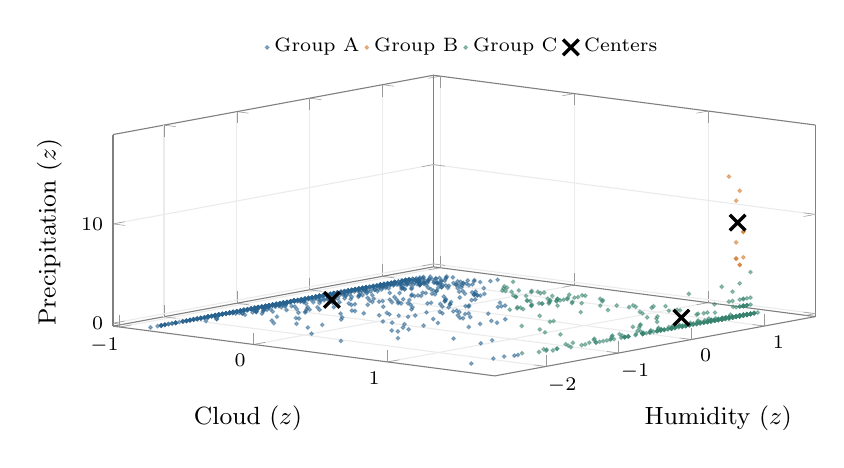
\begin{tikzpicture}
\begin{axis}[width=10.5cm,height=5.4cm,view={40}{22},xlabel={Cloud ($z$)},ylabel={Humidity ($z$)},zlabel={Precipitation ($z$)},legend style={at={(0.5,1.025)},anchor=south,legend columns=4},xmin=-1.05,xmax=1.8,ymin=-2.7,ymax=1.7,zmin=-0.3,zmax=19]
\addplot3[only marks,mark=*,mark size=0.65pt,color=cA,opacity=0.48] coordinates {
(0.59547,-0.45348,-0.11259)
(-0.16561,0.03995,-0.11259)
(-0.48849,0.63208,-0.11259)
(-0.81137,0.92814,-0.11259)
(-0.46542,0.97748,-0.11259)
(-0.53461,1.22420,-0.11259)
(-0.48849,1.22420,-0.11259)
(-0.48849,1.07617,-0.11259)
(-0.62687,0.48405,-0.11259)
(-0.48849,0.87879,-0.11259)
(-0.32705,0.03995,-0.11259)
(-0.81137,0.53339,-0.11259)
(-0.71912,0.43470,-0.11259)
(-0.51155,1.27354,-0.11259)
(-0.41930,1.42157,-0.11259)
(-0.14254,0.18799,-0.11259)
(-0.16561,-0.00939,-0.11259)
(-0.30398,-0.15742,-0.11259)
(-0.46542,-0.45348,-0.11259)
(-0.60380,-0.50282,-0.11259)
(-0.46542,0.08930,-0.11259)
(-0.05029,0.08930,-0.11259)
(-0.64993,0.82945,-0.11259)
(-0.71912,1.27354,-0.11259)
(-0.81137,1.07617,-0.11259)
(-0.78831,1.02683,-0.11259)
(-0.81137,0.73076,-0.11259)
(-0.81137,0.73076,-0.11259)
(-0.81137,0.43470,-0.11259)
(-0.81137,0.58273,-0.11259)
(-0.81137,0.48405,-0.11259)
(-0.81137,0.18799,-0.11259)
(-0.81137,0.33602,-0.11259)
(-0.81137,0.53339,-0.11259)
(-0.71912,1.12551,-0.11259)
(-0.64993,0.78011,-0.11259)
(-0.71912,0.28667,-0.11259)
(-0.67299,-0.30545,-0.11259)
(-0.60380,-0.50282,-0.11259)
(0.06502,-0.60151,-0.11259)
(-0.53461,-0.94692,-0.11259)
(-0.21173,-1.09495,-0.11259)
(-0.64993,-1.24298,-0.11259)
(-0.78831,-1.19363,-0.11259)
(-0.81137,-1.19363,-0.11259)
(-0.81137,-0.65086,-0.11259)
(-0.76524,-0.50282,-0.11259)
(-0.81137,-0.40414,-0.11259)
(-0.81137,-0.35479,-0.11259)
(-0.81137,-0.10808,-0.11259)
(-0.81137,0.38536,-0.11259)
(-0.81137,0.58273,-0.11259)
(-0.81137,0.73076,-0.11259)
(-0.74218,0.92814,-0.11259)
(-0.74218,0.92814,-0.11259)
(-0.69605,0.87879,-0.11259)
(-0.74218,0.92814,-0.11259)
(-0.74218,0.92814,-0.11259)
(-0.67299,1.27354,-0.11259)
(-0.81137,0.33602,-0.11259)
(-0.74218,-0.10808,-0.11259)
(-0.78831,-0.89757,-0.11259)
(-0.71912,-1.14429,-0.11259)
(-0.74218,-1.19363,-0.11259)
(-0.69605,-1.29232,-0.11259)
(-0.71912,-1.34166,-0.11259)
(-0.76524,-1.29232,-0.11259)
(-0.81137,-1.24298,-0.11259)
(-0.81137,-0.99626,-0.11259)
(-0.81137,-0.60151,-0.11259)
(-0.81137,-0.20676,-0.11259)
(-0.81137,0.13864,-0.11259)
(-0.81137,0.58273,-0.11259)
(-0.81137,0.73076,-0.11259)
(-0.81137,0.63208,-0.11259)
(-0.81137,0.58273,-0.11259)
(-0.78831,0.82945,-0.11259)
(-0.71912,0.87879,-0.11259)
(-0.76524,0.92814,-0.11259)
(-0.78831,1.07617,-0.11259)
(-0.71912,1.17486,-0.11259)
(-0.71912,0.87879,-0.11259)
(-0.71912,0.28667,-0.11259)
(-0.78831,-0.30545,-0.11259)
(-0.81137,-0.65086,-0.11259)
(-0.81137,-0.70020,-0.11259)
(-0.78831,-0.79889,-0.11259)
(-0.81137,-0.74954,-0.11259)
(-0.81137,-0.74954,-0.11259)
(-0.81137,-0.65086,-0.11259)
(-0.81137,-0.79889,-0.11259)
(-0.81137,-0.50282,-0.11259)
(-0.81137,-0.05873,-0.11259)
(-0.81137,0.23733,-0.11259)
(-0.81137,0.78011,-0.11259)
(-0.81137,0.92814,-0.11259)
(-0.81137,0.82945,-0.11259)
(-0.81137,0.92814,-0.11259)
(-0.81137,0.87879,-0.11259)
(-0.71912,1.07617,-0.11259)
(-0.81137,0.87879,-0.11259)
(-0.81137,0.53339,-0.11259)
(-0.81137,0.08930,-0.11259)
(-0.35011,-0.15742,-0.11259)
(-0.81137,-0.50282,-0.11259)
(0.24953,-0.25611,-0.11259)
(0.22647,-0.65086,-0.11259)
(0.06502,-0.70020,-0.11259)
(-0.81137,-0.94692,-0.11259)
(-0.76524,-1.14429,-0.11259)
(-0.14254,0.63208,-0.11259)
(-0.76524,0.48405,-0.11259)
(-0.44236,0.43470,-0.11259)
(-0.74218,0.73076,-0.11259)
(-0.18867,0.68142,-0.11259)
(-0.14254,0.63208,-0.11259)
(-0.74218,0.18799,-0.11259)
(0.13421,-0.15742,-0.11259)
(-0.37317,0.03995,-0.11259)
(0.34178,-0.10808,-0.11259)
(-0.44236,-0.25611,-0.11259)
(-0.39624,0.23733,-0.11259)
(-0.05029,0.08930,-0.11259)
(-0.44236,0.28667,-0.11259)
(-0.48849,0.78011,-0.11259)
(-0.62687,1.02683,-0.11259)
(-0.48849,1.07617,-0.11259)
(-0.39624,0.28667,-0.11259)
(-0.32705,-0.10808,-0.11259)
(-0.25786,-0.10808,-0.11259)
(-0.14254,-0.25611,-0.11259)
(-0.09642,-0.35479,-0.11259)
(-0.58074,-0.45348,-0.11259)
(-0.69605,-0.45348,-0.11259)
(-0.81137,-0.35479,-0.11259)
(-0.81137,-0.10808,-0.11259)
(-0.71912,0.33602,-0.11259)
(-0.78831,0.48405,-0.11259)
(-0.81137,0.33602,-0.11259)
(-0.81137,0.68142,-0.11259)
(-0.51155,0.87879,-0.11259)
(0.13421,0.43470,-0.11259)
(-0.09642,0.18799,-0.11259)
(-0.28092,-0.15742,-0.11259)
(0.52628,-0.40414,-0.11259)
(-0.46542,-0.50282,-0.11259)
(0.08809,-0.30545,-0.11259)
(-0.69605,-0.15742,-0.11259)
(-0.67299,0.23733,-0.11259)
(-0.62687,0.97748,-0.11259)
(-0.39624,0.82945,-0.11259)
(-0.78831,0.87879,-0.11259)
(-0.81137,0.87879,-0.11259)
(-0.71912,1.02683,-0.11259)
(-0.64993,1.07617,-0.11259)
(-0.81137,1.02683,-0.11259)
(-0.74218,1.07617,-0.11259)
(-0.78831,1.17486,-0.11259)
(-0.23479,0.78011,-0.11259)
(-0.11948,0.63208,-0.11259)
(-0.05029,0.38536,-0.11259)
(-0.60380,0.48405,-0.11259)
(-0.09642,0.03995,-0.11259)
(-0.64993,-0.00939,-0.11259)
(-0.51155,-0.45348,-0.11259)
(-0.41930,-0.15742,-0.11259)
(-0.76524,-0.20676,-0.11259)
(-0.76524,0.33602,-0.11259)
(-0.74218,0.58273,-0.11259)
(-0.81137,0.82945,-0.11259)
(-0.41930,1.07617,-0.11259)
(-0.69605,0.97748,-0.11259)
(-0.58074,0.92814,-0.11259)
(-0.64993,0.78011,-0.11259)
(-0.78831,0.58273,-0.11259)
(-0.81137,0.33602,-0.11259)
(-0.81137,0.23733,-0.11259)
(-0.81137,0.33602,-0.11259)
(-0.81137,0.13864,-0.11259)
(-0.81137,-0.94692,-0.11259)
(-0.81137,-1.63773,-0.11259)
(-0.81137,-1.83510,-0.11259)
(-0.81137,-1.83510,-0.11259)
(-0.81137,-2.03247,-0.11259)
(-0.81137,-2.37788,-0.11259)
(-0.81137,-2.37788,-0.11259)
(1.44880,-2.37788,-0.11259)
(-0.81137,-2.32854,-0.11259)
(-0.81137,-2.18050,-0.11259)
(-0.81137,-2.03247,-0.11259)
(0.31872,-1.39101,-0.11259)
(-0.81137,-0.94692,-0.11259)
(-0.81137,-0.94692,-0.11259)
(-0.81137,-1.14429,-0.11259)
(-0.81137,-0.99626,-0.11259)
(-0.81137,-1.04560,-0.11259)
(-0.81137,-0.89757,-0.11259)
(-0.81137,-0.65086,-0.11259)
(-0.81137,-0.65086,-0.11259)
(-0.81137,-0.65086,-0.11259)
(-0.81137,-0.70020,-0.11259)
(-0.81137,-0.84823,-0.11259)
(-0.81137,-1.14429,-0.11259)
(-0.81137,-1.48970,-0.11259)
(-0.81137,-1.58838,-0.11259)
(-0.81137,-1.53904,-0.11259)
(-0.81137,-1.63773,-0.11259)
(-0.81137,-1.93379,-0.11259)
(-0.71912,-2.03247,-0.11259)
(-0.78831,-1.88444,-0.11259)
(-0.81137,-2.08182,-0.11259)
(-0.81137,-2.13116,-0.11259)
(-0.81137,-2.13116,-0.11259)
(-0.69605,0.13864,-0.11259)
(-0.71912,-0.10808,-0.11259)
(-0.48849,-0.20676,-0.11259)
(0.08809,0.08930,-0.11259)
(0.06502,0.13864,-0.11259)
(-0.74218,0.23733,-0.11259)
(-0.64993,-0.05873,-0.11259)
(-0.21173,-0.15742,-0.11259)
(0.34178,-0.45348,-0.11259)
(-0.32705,-0.74954,-0.11259)
(-0.78831,-0.79889,-0.11259)
(0.22647,-1.04560,-0.11259)
(0.77998,-1.39101,-0.11259)
(0.52628,-1.68707,-0.11259)
(0.31872,-0.45348,-0.11259)
(0.34178,-0.79889,-0.11259)
(-0.64993,-0.60151,-0.11259)
(0.24953,-0.35479,-0.11259)
(-0.28092,-0.40414,-0.11259)
(-0.74218,-0.15742,-0.11259)
(-0.76524,0.08930,-0.11259)
(-0.81137,0.43470,-0.11259)
(-0.16561,0.23733,-0.11259)
(-0.39624,-0.00939,-0.11259)
(-0.81137,0.33602,-0.11259)
(-0.16561,0.63208,-0.11259)
(0.06502,0.08930,-0.11259)
(0.34178,-0.35479,-0.11259)
(-0.11948,-0.65086,-0.11259)
(-0.07335,-0.70020,-0.11259)
(0.34178,-0.99626,-0.11259)
(-0.30398,-0.94692,-0.11259)
(-0.60380,-0.99626,-0.11259)
(0.54935,-0.60151,-0.11259)
(-0.39624,-0.40414,-0.11259)
(-0.30398,0.73076,-0.11259)
(-0.71912,0.87879,-0.11259)
(-0.64993,0.78011,-0.11259)
(-0.48849,0.73076,-0.11259)
(-0.53461,0.28667,-0.11259)
(0.01890,-0.05873,-0.11259)
(0.13421,-0.20676,-0.11259)
(-0.41930,-0.20676,-0.11259)
(-0.67299,-0.40414,-0.11259)
(-0.71912,-0.35479,-0.11259)
(-0.81137,-0.00939,-0.11259)
(-0.81137,0.18799,-0.11259)
(-0.81137,0.53339,-0.11259)
(-0.81137,0.68142,-0.11259)
(-0.71912,0.97748,-0.11259)
(-0.60380,0.92814,-0.11259)
(-0.64993,0.78011,-0.11259)
(-0.71912,0.73076,-0.11259)
(-0.71912,0.87879,-0.11259)
(-0.76524,0.92814,-0.11259)
(-0.81137,1.12551,-0.11259)
(-0.76524,0.73076,-0.11259)
(-0.76524,0.13864,-0.11259)
(-0.74218,-0.30545,-0.11259)
(-0.21173,-0.79889,-0.11259)
(-0.71912,-1.19363,-0.11259)
(0.36484,-1.24298,-0.11259)
(-0.71912,-1.34166,-0.11259)
(-0.39624,-1.39101,-0.11259)
(0.06502,-1.04560,-0.11259)
(-0.62687,-0.10808,-0.11259)
(-0.48849,0.78011,-0.11259)
(-0.81137,0.63208,-0.11259)
(-0.78831,0.63208,-0.11259)
(-0.76524,0.87879,-0.11259)
(-0.81137,0.53339,-0.11259)
(-0.35011,0.43470,-0.11259)
(-0.81137,0.87879,-0.11259)
(-0.81137,0.73076,-0.11259)
(-0.81137,0.92814,-0.11259)
(-0.48849,0.97748,-0.11259)
(-0.44236,0.58273,-0.11259)
(-0.74218,-0.30545,-0.11259)
(-0.81137,-0.79889,-0.11259)
(-0.81137,-1.19363,-0.11259)
(-0.81137,-1.53904,-0.11259)
(-0.81137,-1.68707,-0.11259)
(-0.81137,-1.83510,-0.11259)
(-0.81137,-2.08182,-0.11259)
(-0.81137,-1.98313,-0.11259)
(-0.71912,-1.88444,-0.11259)
(-0.81137,-1.14429,-0.11259)
(-0.81137,-0.65086,-0.11259)
(-0.81137,-0.35479,-0.11259)
(-0.81137,-0.45348,-0.11259)
(-0.81137,-0.10808,-0.11259)
(-0.81137,-0.00939,-0.11259)
(-0.81137,0.13864,-0.11259)
(-0.81137,0.08930,-0.11259)
(-0.81137,-0.00939,-0.11259)
(-0.78831,-0.15742,-0.11259)
(-0.78831,0.28667,-0.11259)
(-0.81137,0.33602,-0.11259)
(-0.81137,0.63208,-0.11259)
(-0.81137,0.53339,-0.11259)
(-0.81137,0.03995,-0.11259)
(-0.55768,-0.94692,-0.11259)
(-0.81137,-1.14429,-0.11259)
(-0.81137,-1.24298,-0.11259)
(-0.81137,-1.24298,-0.11259)
(-0.78831,-1.53904,-0.11259)
(-0.51155,-1.44035,-0.11259)
(-0.11948,-1.53904,-0.11259)
(0.36484,-1.39101,-0.11259)
(-0.16561,-1.19363,-0.11259)
(-0.62687,-1.09495,-0.11259)
(-0.23479,0.73076,-0.11259)
(-0.14254,0.18799,-0.11259)
(-0.81137,-0.79889,-0.11259)
(-0.78831,-1.04560,-0.11259)
(-0.76524,-1.48970,-0.11259)
(-0.74218,-1.48970,-0.11259)
(-0.78831,-1.73641,-0.11259)
(-0.81137,-1.78576,-0.11259)
(-0.81137,-1.78576,-0.11259)
(-0.81137,-0.94692,-0.11259)
(-0.81137,-0.89757,-0.11259)
(-0.81137,-0.50282,-0.11259)
(-0.81137,-0.20676,-0.11259)
(-0.81137,-0.30545,-0.11259)
(-0.81137,-0.65086,-0.11259)
(-0.81137,-0.00939,-0.11259)
(-0.81137,0.53339,-0.11259)
(-0.81137,0.23733,-0.11259)
(-0.81137,0.08930,-0.11259)
(-0.81137,0.28667,-0.11259)
(-0.81137,0.68142,-0.11259)
(-0.78831,0.82945,-0.11259)
(-0.69605,1.22420,-0.11259)
(-0.81137,0.43470,-0.11259)
(-0.81137,-0.84823,-0.11259)
(-0.81137,-1.24298,-0.11259)
(-0.81137,-1.44035,-0.11259)
(-0.81137,-1.58838,-0.11259)
(-0.81137,-1.73641,-0.11259)
(-0.81137,-1.68707,-0.11259)
(-0.81137,-1.73641,-0.11259)
(-0.81137,-1.73641,-0.11259)
(-0.81137,-1.53904,-0.11259)
(-0.81137,-0.79889,-0.11259)
(-0.81137,-0.30545,-0.11259)
(-0.78831,0.43470,-0.11259)
(-0.53461,0.87879,-0.11259)
(-0.60380,0.92814,-0.11259)
(-0.76524,0.97748,-0.11259)
(-0.81137,0.97748,-0.11259)
(-0.81137,0.82945,-0.11259)
(-0.78831,0.68142,-0.11259)
(-0.76524,-0.05873,-0.11259)
(-0.78831,-0.55217,-0.11259)
(-0.76524,-0.94692,-0.11259)
(-0.76524,-0.94692,-0.11259)
(-0.76524,-0.99626,-0.11259)
(-0.81137,-1.29232,-0.11259)
(-0.81137,-1.44035,-0.11259)
(-0.81137,-1.24298,-0.11259)
(-0.81137,-0.55217,-0.11259)
(-0.81137,-0.05873,-0.11259)
(-0.81137,0.28667,-0.11259)
(-0.81137,0.28667,-0.11259)
(-0.81137,0.18799,-0.11259)
(-0.81137,0.23733,-0.11259)
(-0.81137,-0.25611,-0.11259)
(-0.81137,-0.20676,-0.11259)
(-0.81137,-0.15742,-0.11259)
(-0.81137,-0.30545,-0.11259)
(-0.81137,-0.70020,-0.11259)
(-0.81137,-0.35479,-0.11259)
(-0.71912,-0.40414,-0.11259)
(-0.81137,-0.30545,-0.11259)
(-0.81137,-0.15742,-0.11259)
(-0.81137,-0.94692,-0.11259)
(-0.81137,-1.19363,-0.11259)
(-0.81137,-1.34166,-0.11259)
(-0.81137,-1.53904,-0.11259)
(-0.78831,-1.78576,-0.11259)
(-0.81137,-1.73641,-0.11259)
(-0.81137,-1.88444,-0.11259)
(-0.71912,-1.88444,-0.11259)
(-0.81137,-1.98313,-0.11259)
(-0.81137,-1.48970,-0.11259)
(-0.81137,-1.14429,-0.11259)
(-0.81137,-0.65086,-0.11259)
(-0.81137,-0.89757,-0.11259)
(0.98754,-1.24298,-0.11259)
(1.42574,-1.88444,-0.11259)
(1.42574,-2.03247,-0.11259)
(1.44880,-1.78576,-0.11259)
(1.44880,-1.73641,-0.11259)
(0.13421,-0.35479,-0.11259)
(-0.81137,0.92814,-0.11259)
(-0.81137,0.87879,-0.11259)
(-0.78831,0.58273,-0.11259)
(-0.81137,0.53339,-0.11259)
(-0.81137,0.82945,-0.11259)
(-0.81137,0.28667,-0.11259)
(-0.81137,-0.30545,-0.11259)
(-0.81137,-0.50282,-0.11259)
(-0.81137,-0.65086,-0.11259)
(-0.81137,-0.74954,-0.11259)
(-0.78831,-0.74954,-0.11259)
(-0.69605,-0.89757,-0.11259)
(-0.81137,-0.79889,-0.11259)
(-0.78831,-0.50282,-0.11259)
(-0.67299,-0.00939,-0.11259)
(-0.81137,-0.15742,-0.11259)
(-0.81137,0.33602,-0.11259)
(-0.81137,0.18799,-0.11259)
(-0.76524,0.23733,-0.11259)
(-0.67299,0.73076,-0.11259)
(-0.64993,0.97748,-0.11259)
(-0.74218,0.82945,-0.11259)
(-0.81137,0.33602,-0.11259)
(-0.81137,-0.00939,-0.11259)
(-0.81137,-0.40414,-0.11259)
(-0.81137,0.18799,-0.11259)
(-0.81137,0.58273,-0.11259)
(-0.81137,0.18799,-0.11259)
(-0.81137,-0.50282,-0.11259)
(-0.81137,-0.99626,-0.11259)
(-0.81137,-1.14429,-0.11259)
(-0.81137,-1.24298,-0.11259)
(-0.81137,-1.48970,-0.11259)
(-0.81137,-1.29232,-0.11259)
(-0.81137,-1.34166,-0.11259)
(-0.81137,-1.09495,-0.11259)
(-0.81137,-0.25611,-0.11259)
(-0.81137,-0.00939,-0.11259)
(-0.81137,0.33602,-0.11259)
(-0.81137,0.13864,-0.11259)
(-0.81137,0.03995,-0.11259)
(-0.81137,-0.05873,-0.11259)
(-0.81137,-0.05873,-0.11259)
(-0.81137,-0.30545,-0.11259)
(-0.81137,-0.40414,-0.11259)
(-0.81137,-0.40414,-0.11259)
(-0.81137,-0.30545,-0.11259)
(-0.81137,-0.15742,-0.11259)
(-0.81137,-0.35479,-0.11259)
(-0.76524,-0.45348,-0.11259)
(-0.81137,-0.30545,-0.11259)
(-0.81137,-0.35479,-0.11259)
(-0.81137,-0.89757,-0.11259)
(-0.81137,-1.09495,-0.11259)
(-0.81137,-1.09495,-0.11259)
(-0.81137,-1.19363,-0.11259)
(-0.81137,-1.14429,-0.11259)
(-0.81137,-1.19363,-0.11259)
(-0.81137,-1.29232,-0.11259)
(-0.51155,-1.14429,-0.11259)
(-0.76524,-0.60151,-0.11259)
(-0.81137,-0.50282,-0.11259)
(-0.74218,-0.30545,-0.11259)
(0.54935,-0.25611,-0.11259)
(-0.53461,1.02683,-0.11259)
(-0.81137,0.97748,-0.11259)
(-0.39624,0.87879,-0.11259)
(-0.62687,0.92814,-0.11259)
(-0.69605,0.68142,-0.11259)
(-0.69605,0.43470,-0.11259)
(-0.81137,0.08930,-0.11259)
(-0.81137,-0.15742,-0.11259)
(-0.78831,-0.60151,-0.11259)
(-0.78831,-0.65086,-0.11259)
(-0.78831,-0.35479,-0.11259)
(-0.60380,-0.25611,-0.11259)
(-0.02723,-0.05873,-0.11259)
(0.18034,-0.20676,-0.11259)
(-0.51155,-1.04560,-0.11259)
(-0.37317,-1.39101,-0.11259)
(-0.81137,-1.53904,-0.11259)
(-0.81137,-1.68707,-0.11259)
(-0.81137,-1.73641,-0.11259)
(-0.81137,-1.24298,-0.11259)
(-0.81137,-0.74954,-0.11259)
(-0.81137,-0.45348,-0.11259)
(-0.81137,-0.20676,-0.11259)
(-0.81137,-0.10808,-0.11259)
(-0.81137,-0.35479,-0.11259)
(-0.81137,-0.30545,-0.11259)
(-0.81137,-0.00939,-0.11259)
(-0.81137,0.23733,-0.11259)
(-0.81137,-0.40414,-0.11259)
(-0.81137,-0.20676,-0.11259)
(-0.81137,0.28667,-0.11259)
(-0.81137,0.28667,-0.11259)
(-0.81137,0.23733,-0.11259)
(-0.81137,-0.10808,-0.11259)
(-0.81137,-0.65086,-0.11259)
(-0.81137,-1.34166,-0.11259)
(-0.81137,-1.73641,-0.11259)
(-0.81137,-2.08182,-0.11259)
(-0.81137,-2.42722,-0.11259)
(-0.81137,-2.42722,-0.11259)
(-0.81137,-2.62460,-0.11259)
(-0.81137,-2.52591,-0.11259)
(-0.81137,-1.98313,-0.11259)
(-0.81137,-1.73641,-0.11259)
(-0.81137,-0.99626,-0.11259)
(-0.81137,-0.40414,-0.11259)
(-0.81137,0.13864,-0.11259)
(-0.81137,0.53339,-0.11259)
(-0.74218,0.92814,-0.11259)
(-0.41930,1.02683,-0.11259)
(-0.25786,0.38536,-0.11259)
(-0.78831,0.53339,-0.11259)
(-0.76524,0.73076,-0.11259)
(-0.60380,0.58273,-0.11259)
(-0.74218,0.63208,-0.11259)
(-0.76524,0.63208,-0.11259)
(-0.81137,0.63208,-0.11259)
(-0.81137,-0.35479,-0.11259)
(-0.81137,-1.19363,-0.11259)
(-0.81137,-1.88444,-0.11259)
(-0.81137,-1.93379,-0.11259)
(-0.81137,-2.03247,-0.11259)
(-0.81137,-2.22985,-0.11259)
(-0.81137,-2.27919,-0.11259)
(-0.81137,-2.27919,-0.11259)
(-0.81137,-2.13116,-0.11259)
(-0.81137,-1.78576,-0.11259)
(-0.81137,-1.29232,-0.11259)
(-0.81137,-0.84823,-0.11259)
(-0.81137,-0.70020,-0.11259)
(-0.81137,-0.79889,-0.11259)
(-0.81137,-0.60151,-0.11259)
(-0.81137,-0.74954,-0.11259)
(-0.81137,-0.55217,-0.11259)
(-0.81137,0.03995,-0.11259)
(-0.81137,0.03995,-0.11259)
(-0.81137,-0.30545,-0.11259)
(-0.81137,-0.55217,-0.11259)
(-0.81137,-0.70020,-0.11259)
(-0.81137,-0.84823,-0.11259)
(-0.81137,-0.74954,-0.11259)
(-0.81137,-0.99626,-0.11259)
(-0.81137,-1.39101,-0.11259)
(-0.81137,-1.98313,-0.11259)
(-0.81137,-1.98313,-0.11259)
(-0.81137,-1.93379,-0.11259)
(-0.81137,-2.03247,-0.11259)
(-0.81137,-2.08182,-0.11259)
(-0.81137,-2.13116,-0.11259)
(-0.81137,-1.98313,-0.11259)
(-0.81137,-1.44035,-0.11259)
(-0.81137,-0.89757,-0.11259)
(-0.81137,-0.30545,-0.11259)
(-0.81137,-0.30545,-0.11259)
(-0.81137,-0.10808,-0.11259)
(-0.81137,-0.10808,-0.11259)
(-0.81137,0.13864,-0.11259)
(-0.81137,-0.05873,-0.11259)
(-0.81137,-0.20676,-0.11259)
(-0.81137,-0.05873,-0.11259)
(-0.81137,-0.05873,-0.11259)
(-0.81137,-0.10808,-0.11259)
(-0.78831,0.08930,-0.11259)
(-0.81137,-0.00939,-0.11259)
(-0.81137,0.08930,-0.11259)
(-0.81137,-0.89757,-0.11259)
(-0.81137,-1.44035,-0.11259)
(-0.81137,-1.48970,-0.11259)
(-0.81137,-1.68707,-0.11259)
(-0.81137,-1.78576,-0.11259)
(-0.81137,-1.88444,-0.11259)
(-0.81137,-1.83510,-0.11259)
(-0.81137,-1.83510,-0.11259)
(-0.81137,-1.68707,-0.11259)
(-0.81137,-1.19363,-0.11259)
(-0.81137,-0.94692,-0.11259)
(-0.81137,-0.65086,-0.11259)
(-0.81137,0.03995,-0.11259)
(-0.81137,0.08930,-0.11259)
(-0.81137,-0.05873,-0.11259)
(-0.78831,0.53339,-0.11259)
(-0.81137,-0.00939,-0.11259)
(-0.81137,-0.15742,-0.11259)
(-0.81137,-0.05873,-0.11259)
(-0.81137,-0.10808,-0.11259)
(-0.78831,0.03995,-0.11259)
(-0.78831,0.08930,-0.11259)
(-0.78831,-0.00939,-0.11259)
(-0.81137,-0.10808,-0.11259)
(-0.81137,-0.50282,-0.11259)
(-0.81137,-1.19363,-0.11259)
(-0.81137,-1.68707,-0.11259)
(-0.81137,-1.93379,-0.11259)
(-0.81137,-2.08182,-0.11259)
(-0.81137,-2.27919,-0.11259)
(-0.81137,-2.42722,-0.11259)
(-0.81137,-2.42722,-0.11259)
(-0.81137,-2.27919,-0.11259)
(-0.81137,-1.68707,-0.11259)
(-0.81137,-1.48970,-0.11259)
(-0.81137,-1.29232,-0.11259)
(-0.81137,-0.89757,-0.11259)
(-0.81137,-0.89757,-0.11259)
(-0.81137,-0.70020,-0.11259)
(-0.81137,-0.55217,-0.11259)
(-0.81137,-0.84823,-0.11259)
(-0.81137,-0.84823,-0.11259)
(-0.81137,-0.84823,-0.11259)
(-0.81137,-0.65086,-0.11259)
(-0.78831,-0.10808,-0.11259)
(-0.81137,-0.15742,-0.11259)
(-0.81137,0.08930,-0.11259)
(-0.81137,0.08930,-0.11259)
(-0.74218,-0.45348,-0.11259)
(-0.74218,-0.65086,-0.11259)
(-0.78831,-0.84823,-0.11259)
(-0.81137,-1.14429,-0.11259)
(-0.76524,-1.24298,-0.11259)
(-0.81137,-1.34166,-0.11259)
(-0.81137,-1.24298,-0.11259)
(-0.81137,-0.70020,-0.11259)
(-0.81137,-0.35479,-0.11259)
(-0.81137,0.18799,-0.11259)
(-0.78831,0.63208,-0.11259)
(-0.81137,0.63208,-0.11259)
(-0.81137,0.82945,-0.11259)
(-0.71912,1.12551,-0.11259)
(-0.81137,0.73076,-0.11259)
(-0.71912,0.82945,-0.11259)
(-0.78831,0.68142,-0.11259)
(-0.71912,0.73076,-0.11259)
(-0.69605,0.73076,-0.11259)
(-0.60380,0.78011,-0.11259)
(-0.67299,0.82945,-0.11259)
(-0.41930,1.32289,-0.11259)
(-0.14254,0.73076,-0.11259)
(-0.71912,-0.05873,-0.11259)
(-0.76524,-0.89757,-0.11259)
(-0.81137,-1.09495,-0.11259)
(-0.71912,-1.34166,-0.11259)
(-0.76524,-1.53904,-0.11259)
(-0.64993,-1.39101,-0.11259)
(-0.71912,-1.24298,-0.11259)
(-0.81137,-1.19363,-0.11259)
(-0.81137,-0.94692,-0.11259)
(-0.64993,-0.15742,-0.11259)
(-0.71912,0.08930,-0.11259)
(-0.78831,0.63208,-0.11259)
(-0.78831,0.63208,-0.11259)
(-0.74218,0.68142,-0.11259)
(-0.67299,0.87879,-0.11259)
(-0.64993,0.87879,-0.11259)
(-0.74218,0.92814,-0.11259)
(0.22647,0.23733,-0.11259)
(-0.69605,-0.40414,-0.11259)
(-0.76524,-0.60151,-0.11259)
(-0.78831,-0.89757,-0.11259)
(-0.71912,-0.94692,-0.11259)
(-0.78831,-1.04560,-0.11259)
(-0.76524,-1.14429,-0.11259)
(-0.81137,-1.19363,-0.11259)
(-0.81137,-0.89757,-0.11259)
(-0.81137,-0.25611,-0.11259)
(-0.81137,0.28667,-0.11259)
(-0.74218,0.18799,-0.11259)
(0.22647,0.28667,-0.11259)
(-0.60380,0.48405,-0.11259)
(-0.81137,0.23733,-0.11259)
(-0.81137,0.33602,-0.11259)
(-0.81137,0.28667,-0.11259)
(-0.81137,0.18799,-0.11259)
(-0.81137,0.33602,-0.11259)
(-0.81137,0.13864,-0.11259)
(-0.81137,0.13864,-0.11259)
(-0.69605,0.18799,-0.11259)
(-0.81137,0.68142,-0.11259)
(-0.81137,0.87879,-0.11259)
(-0.81137,0.73076,-0.11259)
(-0.81137,0.28667,-0.11259)
(-0.81137,-0.45348,-0.11259)
(-0.81137,-1.04560,-0.11259)
(-0.81137,-1.53904,-0.11259)
(-0.81137,-1.63773,-0.11259)
(-0.81137,-1.63773,-0.11259)
(-0.81137,-1.53904,-0.11259)
(-0.81137,-1.34166,-0.11259)
(-0.81137,-0.79889,-0.11259)
(-0.81137,-0.15742,-0.11259)
(-0.81137,-0.00939,-0.11259)
(-0.81137,0.43470,-0.11259)
(-0.78831,0.48405,-0.11259)
(-0.81137,-0.30545,-0.11259)
(-0.81137,-1.14429,-0.11259)
(-0.81137,-0.65086,-0.11259)
(-0.71912,-0.45348,-0.11259)
(-0.81137,-0.35479,-0.11259)
(-0.81137,-0.10808,-0.11259)
(-0.81137,0.03995,-0.11259)
(-0.76524,0.18799,-0.11259)
(-0.81137,0.13864,-0.11259)
(-0.81137,0.08930,-0.11259)
(-0.81137,-0.35479,-0.11259)
(-0.81137,-0.79889,-0.11259)
(-0.81137,-1.04560,-0.11259)
(-0.81137,-1.19363,-0.11259)
(-0.81137,-1.19363,-0.11259)
(-0.78831,-1.24298,-0.11259)
(-0.81137,-1.34166,-0.11259)
(-0.81137,-1.39101,-0.11259)
(-0.81137,-1.34166,-0.11259)
(-0.81137,-1.04560,-0.11259)
(-0.81137,-0.50282,-0.11259)
(-0.67299,0.78011,-0.11259)
(-0.64993,0.78011,-0.11259)
(-0.81137,0.48405,-0.11259)
(-0.69605,0.63208,-0.11259)
(-0.23479,0.63208,-0.11259)
(-0.05029,0.43470,-0.11259)
(0.22647,0.33602,-0.11259)
(-0.76524,0.68142,-0.11259)
(-0.62687,1.07617,-0.11259)
(-0.67299,0.87879,-0.11259)
(-0.78831,0.18799,-0.11259)
(-0.67299,-0.35479,-0.11259)
(-0.69605,-0.60151,-0.11259)
(-0.76524,-0.99626,-0.11259)
(-0.81137,-1.24298,-0.11259)
(-0.81137,-1.39101,-0.11259)
(-0.81137,-1.14429,-0.11259)
(-0.81137,-1.04560,-0.11259)
(-0.81137,-0.35479,-0.11259)
(-0.81137,0.18799,-0.11259)
(-0.81137,0.38536,-0.11259)
(-0.81137,0.33602,-0.11259)
(-0.81137,0.23733,-0.11259)
(-0.81137,0.33602,-0.11259)
(-0.81137,0.08930,-0.11259)
(-0.81137,-0.55217,-0.11259)
(-0.81137,-0.99626,-0.11259)
(-0.81137,-0.79889,-0.11259)
(-0.81137,-0.70020,-0.11259)
(-0.81137,-0.30545,-0.11259)
(-0.81137,-0.45348,-0.11259)
(-0.71912,-0.99626,-0.11259)
(-0.81137,-0.70020,-0.11259)
(-0.81137,-1.09495,-0.11259)
(-0.81137,-1.39101,-0.11259)
(-0.81137,-1.58838,-0.11259)
(-0.81137,-1.83510,-0.11259)
(-0.81137,-2.08182,-0.11259)
(-0.81137,-2.32854,-0.11259)
(-0.81137,-2.47657,-0.11259)
(-0.81137,-2.47657,-0.11259)
(-0.81137,-2.47657,-0.11259)
(-0.81137,-2.03247,-0.11259)
(-0.81137,-1.93379,-0.11259)
(-0.81137,-1.73641,-0.11259)
(-0.81137,-1.39101,-0.11259)
(-0.76524,-1.09495,-0.11259)
(-0.81137,-1.04560,-0.11259)
(-0.81137,-0.79889,-0.11259)
(-0.81137,-0.50282,-0.11259)
(-0.81137,-0.65086,-0.11259)
(-0.81137,-0.00939,-0.11259)
(-0.81137,-0.05873,-0.11259)
(-0.41930,-0.05873,-0.11259)
(-0.81137,-0.20676,-0.11259)
(-0.60380,0.03995,-0.11259)
(-0.81137,0.48405,-0.11259)
(-0.78831,-0.10808,-0.11259)
(-0.76524,-0.65086,-0.11259)
(-0.55768,-0.79889,-0.11259)
(0.13421,-1.04560,-0.11259)
(1.01061,-1.44035,-0.11259)
(-0.30398,-0.74954,-0.11259)
(0.24953,-0.20676,-0.11259)
(-0.41930,0.43470,-0.11259)
(-0.74218,0.48405,-0.11259)
(-0.76524,0.43470,-0.11259)
(-0.69605,0.33602,-0.11259)
(-0.16561,0.43470,-0.11259)
(-0.16561,0.63208,-0.11259)
(-0.58074,0.23733,-0.11259)
(-0.76524,0.48405,-0.11259)
(-0.81137,0.58273,-0.11259)
(-0.81137,0.03995,-0.11259)
(-0.78831,-0.60151,-0.11259)
(-0.81137,-1.48970,-0.11259)
(-0.81137,-1.63773,-0.11259)
(-0.81137,-1.93379,-0.11259)
(-0.81137,-2.03247,-0.11259)
(0.34178,-2.13116,-0.11259)
(0.04196,-1.98313,-0.11259)
(-0.37317,-1.73641,-0.11259)
(-0.48849,-1.09495,-0.11259)
(-0.81137,-0.94692,-0.11259)
(-0.74218,-0.25611,-0.11259)
(-0.51155,-0.10808,-0.11259)
(-0.41930,0.23733,-0.11259)
(-0.41930,0.58273,-0.11259)
(-0.62687,0.73076,-0.11259)
(0.04196,-0.40414,-0.11259)
(0.29565,-1.19363,-0.11259)
(-0.81137,-1.39101,-0.11259)
(-0.69605,-1.53904,-0.11259)
(-0.71912,-1.39101,-0.11259)
(-0.74218,-1.48970,-0.11259)
(-0.25786,-1.63773,-0.11259)
(-0.81137,-1.39101,-0.11259)
(-0.78831,-0.94692,-0.11259)
(-0.69605,-0.70020,-0.11259)
(-0.81137,-0.00939,-0.11259)
(-0.81137,0.08930,-0.11259)
(-0.81137,0.43470,-0.11259)
(-0.76524,0.63208,-0.11259)
(-0.37317,0.28667,-0.11259)
(-0.81137,0.73076,-0.11259)
(-0.81137,0.33602,-0.11259)
(-0.81137,0.23733,-0.11259)
(-0.81137,-0.00939,-0.11259)
(-0.81137,0.53339,-0.11259)
(-0.81137,0.78011,-0.11259)
(-0.64993,0.53339,-0.11259)
(-0.78831,0.03995,-0.11259)
(-0.64993,-0.40414,-0.11259)
(-0.09642,-0.79889,-0.11259)
(-0.81137,-0.70020,-0.11259)
(-0.81137,-1.04560,-0.11259)
(-0.81137,-1.39101,-0.11259)
(-0.81137,-1.29232,-0.11259)
(-0.81137,-0.99626,-0.11259)
(-0.81137,-1.04560,-0.11259)
(-0.81137,-0.55217,-0.11259)
(-0.81137,-0.05873,-0.11259)
(-0.81137,0.18799,-0.11259)
(-0.81137,0.38536,-0.11259)
(-0.81137,0.58273,-0.11259)
(-0.81137,0.63208,-0.11259)
(-0.81137,0.58273,-0.11259)
(-0.81137,0.53339,-0.11259)
(-0.76524,0.58273,-0.11259)
(-0.78831,0.97748,-0.11259)
(-0.53461,1.12551,-0.11259)
(-0.55768,1.12551,-0.11259)
(-0.76524,1.02683,-0.11259)
(-0.69605,0.97748,-0.11259)
(-0.67299,1.17486,-0.11259)
(-0.58074,0.53339,-0.11259)
(-0.55768,-0.10808,-0.11259)
(-0.69605,-0.50282,-0.11259)
(-0.81137,-0.79889,-0.11259)
(-0.67299,-0.89757,-0.11259)
(-0.48849,-0.89757,-0.11259)
(-0.48849,-0.70020,-0.11259)
(-0.74218,-0.89757,-0.11259)
(0.57241,-0.79889,-0.11259)
(-0.74218,0.43470,-0.11259)
(-0.37317,0.43470,-0.11259)
(-0.48849,0.97748,-0.11259)
(-0.44236,0.78011,-0.11259)
(-0.74218,0.78011,-0.11259)
(-0.74218,0.68142,-0.11259)
(-0.78831,0.63208,-0.11259)
(-0.44236,1.22420,-0.11259)
(-0.28092,0.97748,-0.11259)
(-0.41930,0.58273,-0.11259)
(-0.67299,0.08930,-0.11259)
(-0.81137,0.13864,-0.11259)
(-0.81137,-0.50282,-0.11259)
(-0.81137,-0.70020,-0.11259)
(-0.81137,-0.00939,-0.11259)
(-0.64993,0.53339,-0.11259)
(-0.44236,0.97748,-0.11259)
(-0.46542,1.07617,-0.11259)
(-0.30398,0.68142,-0.11259)
(-0.71912,0.63208,-0.11259)
(-0.53461,0.68142,-0.11259)
(-0.55768,0.87879,-0.11259)
(-0.18867,0.28667,-0.11259)
(-0.64993,-0.25611,-0.11259)
(-0.81137,-0.30545,-0.11259)
(-0.81137,-0.45348,-0.11259)
(-0.81137,-0.40414,-0.11259)
(-0.81137,-0.05873,-0.11259)
(-0.81137,-0.94692,-0.11259)
(-0.81137,-1.19363,-0.11259)
(-0.81137,-1.34166,-0.11259)
(-0.81137,-1.44035,-0.11259)
(-0.81137,-1.68707,-0.11259)
(-0.81137,-1.73641,-0.11259)
(-0.81137,-1.83510,-0.11259)
(-0.81137,-1.83510,-0.11259)
(-0.81137,-1.39101,-0.11259)
(-0.81137,-1.04560,-0.11259)
(-0.81137,-0.89757,-0.11259)
(-0.81137,-0.65086,-0.11259)
(-0.81137,-0.60151,-0.11259)
(-0.81137,-0.55217,-0.11259)
(-0.81137,-0.35479,-0.11259)
(-0.81137,-0.60151,-0.11259)
(-0.81137,-0.45348,-0.11259)
(-0.81137,-0.20676,-0.11259)
(-0.81137,-0.30545,-0.11259)
(-0.81137,-0.55217,-0.11259)
(-0.81137,-0.55217,-0.11259)
(-0.81137,-0.84823,-0.11259)
(-0.81137,-1.04560,-0.11259)
(-0.81137,-0.65086,-0.11259)
(-0.81137,-0.89757,-0.11259)
(-0.81137,-0.94692,-0.11259)
(-0.81137,-1.14429,-0.11259)
(-0.81137,-1.73641,-0.11259)
(-0.81137,-1.48970,-0.11259)
(-0.81137,-1.63773,-0.11259)
(-0.81137,-1.88444,-0.11259)
(-0.81137,-1.88444,-0.11259)
(-0.81137,-1.68707,-0.11259)
(-0.81137,-1.44035,-0.11259)
(-0.81137,-1.58838,-0.11259)
(-0.81137,-1.58838,-0.11259)
(-0.81137,-1.58838,-0.11259)
(-0.44236,-1.63773,-0.11259)
(-0.81137,-1.73641,-0.11259)
(-0.11948,-1.73641,-0.11259)
(-0.81137,-1.63773,-0.11259)
(-0.81137,-1.53904,-0.11259)
(-0.81137,-1.34166,-0.11259)
(-0.81137,-1.09495,-0.11259)
(-0.81137,-0.65086,-0.11259)
(-0.00416,-0.70020,-0.11259)
(-0.60380,-0.84823,-0.11259)
(-0.81137,-0.79889,-0.11259)
(-0.81137,-0.99626,-0.11259)
(-0.78831,-1.34166,-0.11259)
(-0.81137,-1.68707,-0.11259)
(-0.81137,-1.93379,-0.11259)
(-0.81137,-2.08182,-0.11259)
(-0.81137,-2.18050,-0.11259)
(-0.81137,-2.27919,-0.11259)
(-0.81137,-2.47657,-0.11259)
(-0.81137,-2.18050,-0.11259)
(-0.81137,-1.73641,-0.11259)
};
\addlegendentry{Group A}
\addplot3[only marks,mark=*,mark size=0.65pt,color=cB,opacity=0.48] coordinates {
(1.49493,1.07617,22.51536)
(1.49493,1.17486,5.71936)
(1.49493,1.27354,8.28541)
(1.49493,1.07617,14.11736)
(1.49493,1.22420,12.48441)
(1.49493,1.22420,5.01952)
(1.49493,1.17486,11.55130)
(1.49493,1.17486,7.35230)
(1.49493,1.27354,8.28541)
(1.49493,1.27354,5.71936)
(1.49493,1.22420,5.01952)
(1.49493,1.17486,5.71936)
};
\addlegendentry{Group B}
\addplot3[only marks,mark=*,mark size=0.65pt,color=cC,opacity=0.48] coordinates {
(0.31872,0.33602,-0.11259)
(0.34178,0.73076,-0.11259)
(-0.18867,1.12551,-0.11259)
(1.49493,1.07617,-0.11259)
(1.49493,1.07617,-0.11259)
(1.49493,1.07617,-0.11259)
(1.49493,0.63208,-0.11259)
(1.49493,0.28667,-0.11259)
(1.49493,0.13864,-0.11259)
(1.49493,0.23733,-0.11259)
(1.47187,0.43470,-0.11259)
(1.47187,0.58273,-0.11259)
(0.34178,0.63208,-0.11259)
(1.49493,1.02683,-0.11259)
(1.49493,1.22420,-0.11259)
(1.49493,1.32289,-0.11259)
(1.49493,1.22420,-0.11259)
(1.49493,1.17486,-0.11259)
(1.49493,1.32289,-0.11259)
(1.49493,1.12551,-0.11259)
(1.49493,1.02683,-0.11259)
(1.49493,1.07617,-0.11259)
(1.49493,1.27354,-0.11259)
(1.49493,1.32289,-0.11259)
(1.49493,1.17486,-0.11259)
(1.49493,1.07617,-0.11259)
(1.49493,0.97748,-0.11259)
(1.49493,0.87879,-0.11259)
(1.49493,1.22420,-0.11259)
(1.49493,1.17486,-0.11259)
(1.49493,0.78011,-0.11259)
(1.49493,0.68142,-0.11259)
(0.50322,0.87879,-0.11259)
(1.49493,0.97748,-0.11259)
(1.49493,1.12551,-0.11259)
(1.49493,1.17486,-0.11259)
(1.49493,1.27354,-0.11259)
(1.49493,1.12551,-0.11259)
(1.49493,1.12551,-0.11259)
(1.49493,1.17486,-0.11259)
(1.49493,1.22420,-0.11259)
(1.49493,1.27354,1.52036)
(1.49493,1.32289,-0.11259)
(1.49493,1.32289,-0.11259)
(1.49493,1.37223,-0.11259)
(1.49493,1.32289,-0.11259)
(1.49493,1.27354,-0.11259)
(1.49493,1.07617,-0.11259)
(1.49493,0.48405,-0.11259)
(1.49493,-0.65086,-0.11259)
(0.34178,0.82945,-0.11259)
(0.29565,0.92814,-0.11259)
(0.54935,1.07617,-0.11259)
(-0.07335,1.07617,-0.11259)
(1.49493,1.12551,2.45347)
(1.49493,1.07617,-0.11259)
(1.49493,1.22420,-0.11259)
(1.31043,1.22420,-0.11259)
(1.49493,1.22420,-0.11259)
(1.49493,1.17486,-0.11259)
(0.08809,0.87879,-0.11259)
(0.31872,0.53339,-0.11259)
(1.47187,0.53339,-0.11259)
(0.34178,0.97748,-0.11259)
(-0.07335,0.97748,-0.11259)
(0.31872,0.63208,-0.11259)
(1.49493,-0.10808,-0.11259)
(1.49493,0.58273,-0.11259)
(0.24953,0.87879,-0.11259)
(0.31872,1.22420,-0.11259)
(0.48016,1.17486,-0.11259)
(1.49493,0.97748,-0.11259)
(1.49493,1.02683,-0.11259)
(1.49493,0.63208,-0.11259)
(1.49493,0.78011,-0.11259)
(0.06502,0.78011,-0.11259)
(1.49493,0.48405,-0.11259)
(1.49493,0.28667,-0.11259)
(1.49493,0.18799,-0.11259)
(1.49493,0.48405,-0.11259)
(1.49493,0.48405,-0.11259)
(1.49493,0.82945,-0.11259)
(1.49493,0.68142,-0.11259)
(1.49493,0.73076,-0.11259)
(1.49493,0.23733,-0.11259)
(1.49493,0.28667,-0.11259)
(1.49493,1.07617,-0.11259)
(0.71079,0.97748,-0.11259)
(1.03367,-0.60151,-0.11259)
(1.49493,-0.60151,-0.11259)
(0.80304,-0.10808,-0.11259)
(1.14899,0.73076,-0.11259)
(0.64160,0.87879,-0.11259)
(0.77998,1.07617,-0.11259)
(-0.23479,1.17486,-0.11259)
(1.49493,0.97748,-0.11259)
(1.49493,0.82945,-0.11259)
(1.49493,0.97748,-0.11259)
(1.49493,0.73076,-0.11259)
(1.49493,0.78011,-0.11259)
(1.49493,0.63208,-0.11259)
(1.49493,0.68142,-0.11259)
(1.49493,0.78011,-0.11259)
(1.49493,0.58273,-0.11259)
(1.49493,0.87879,-0.11259)
(1.49493,1.12551,-0.11259)
(1.49493,1.12551,-0.11259)
(1.49493,1.07617,-0.11259)
(1.49493,1.07617,-0.11259)
(1.49493,1.27354,-0.11259)
(1.49493,1.17486,-0.11259)
(1.49493,1.27354,-0.11259)
(1.49493,1.27354,-0.11259)
(1.49493,1.27354,-0.11259)
(1.49493,1.22420,-0.11259)
(1.49493,1.27354,-0.11259)
(1.49493,1.22420,-0.11259)
(1.49493,1.12551,-0.11259)
(1.49493,1.27354,-0.11259)
(1.49493,1.17486,-0.11259)
(1.49493,1.27354,-0.11259)
(1.49493,0.97748,-0.11259)
(1.49493,1.22420,-0.11259)
(1.49493,1.02683,-0.11259)
(1.49493,0.92814,-0.11259)
(1.49493,1.32289,0.82052)
(1.49493,1.12551,-0.11259)
(1.49493,1.17486,-0.11259)
(1.49493,1.27354,0.82052)
(1.49493,1.32289,-0.11259)
(1.49493,1.27354,0.82052)
(1.49493,1.22420,-0.11259)
(1.49493,1.22420,0.82052)
(1.49493,1.22420,-0.11259)
(1.49493,1.22420,-0.11259)
(1.49493,1.27354,-0.11259)
(1.49493,1.27354,0.82052)
(1.49493,1.22420,0.82052)
(1.49493,1.12551,-0.11259)
(1.49493,1.07617,-0.11259)
(1.49493,1.12551,-0.11259)
(1.49493,1.12551,-0.11259)
(1.49493,1.07617,-0.11259)
(1.49493,1.37223,-0.11259)
(1.49493,1.22420,-0.11259)
(1.49493,1.22420,-0.11259)
(1.49493,1.22420,-0.11259)
(1.49493,1.22420,-0.11259)
(1.49493,1.27354,0.82052)
(1.49493,1.32289,-0.11259)
(1.49493,1.27354,-0.11259)
(1.49493,1.12551,-0.11259)
(1.49493,1.07617,-0.11259)
(1.49493,1.02683,-0.11259)
(1.49493,1.12551,-0.11259)
(1.49493,0.97748,-0.11259)
(0.34178,0.87879,-0.11259)
(0.20340,0.68142,-0.11259)
(1.49493,0.53339,-0.11259)
(0.34178,0.48405,-0.11259)
(1.49493,0.43470,-0.11259)
(1.49493,0.48405,-0.11259)
(1.49493,0.38536,-0.11259)
(1.49493,0.43470,-0.11259)
(0.34178,0.28667,-0.11259)
(1.49493,-0.35479,-0.11259)
(1.49493,-0.35479,-0.11259)
(1.49493,-0.50282,-0.11259)
(1.49493,1.07617,-0.11259)
(0.20340,1.02683,-0.11259)
(1.49493,-0.55217,-0.11259)
(1.49493,-0.30545,-0.11259)
(1.42574,0.92814,-0.11259)
(1.49493,0.92814,-0.11259)
(0.96448,0.82945,-0.11259)
(1.12592,0.63208,-0.11259)
(1.49493,-1.09495,-0.11259)
(1.42574,-1.34166,-0.11259)
(1.49493,-0.89757,-0.11259)
(1.47187,-0.79889,-0.11259)
(0.34178,0.33602,-0.11259)
(0.34178,0.48405,-0.11259)
(1.49493,-0.74954,-0.11259)
(1.49493,-0.10808,-0.11259)
(1.49493,0.33602,-0.11259)
(1.49493,0.48405,-0.11259)
(1.49493,0.08930,-0.11259)
(1.49493,0.03995,-0.11259)
(1.49493,0.18799,-0.11259)
(1.49493,0.97748,-0.11259)
(0.22647,0.68142,-0.11259)
(1.01061,0.78011,-0.11259)
(0.34178,1.07617,-0.11259)
(1.49493,-0.10808,-0.11259)
(1.49493,-0.10808,-0.11259)
(1.40268,-0.00939,-0.11259)
(0.04196,1.12551,-0.11259)
(0.29565,0.92814,-0.11259)
(-0.11948,0.97748,-0.11259)
(0.34178,1.22420,-0.11259)
(0.71079,0.48405,-0.11259)
(0.36484,0.68142,-0.11259)
(-0.14254,0.97748,-0.11259)
(1.49493,-0.00939,-0.11259)
(1.49493,-0.05873,-0.11259)
(0.82610,1.02683,-0.11259)
(-0.18867,1.07617,-0.11259)
(1.49493,0.97748,-0.11259)
(1.49493,0.73076,-0.11259)
(1.49493,0.18799,-0.11259)
(1.49493,0.48405,-0.11259)
(1.49493,0.87879,-0.11259)
(1.49493,1.22420,1.52036)
(1.49493,1.22420,3.15330)
(1.49493,1.27354,0.82052)
(1.49493,1.37223,4.08641)
(1.49493,1.22420,-0.11259)
(1.47187,1.17486,0.82052)
(1.47187,1.07617,-0.11259)
(1.49493,1.07617,-0.11259)
(1.49493,1.22420,-0.11259)
(1.49493,1.17486,-0.11259)
(1.49493,1.17486,-0.11259)
(1.49493,1.32289,-0.11259)
(1.49493,1.32289,-0.11259)
(1.49493,1.32289,-0.11259)
(1.49493,1.32289,-0.11259)
(1.49493,1.27354,-0.11259)
(1.49493,1.37223,-0.11259)
(1.49493,1.27354,-0.11259)
(1.49493,1.37223,-0.11259)
(1.49493,1.42157,-0.11259)
(1.49493,1.32289,-0.11259)
(1.49493,1.37223,-0.11259)
(1.49493,1.37223,-0.11259)
(1.49493,1.37223,-0.11259)
(1.49493,1.32289,-0.11259)
(1.49493,1.22420,-0.11259)
(1.49493,1.42157,-0.11259)
(1.49493,1.37223,0.82052)
(1.49493,1.37223,-0.11259)
(1.49493,1.17486,-0.11259)
(1.49493,1.07617,-0.11259)
(1.49493,0.87879,-0.11259)
(1.49493,0.92814,-0.11259)
(1.49493,0.87879,-0.11259)
(1.49493,0.87879,-0.11259)
(1.49493,0.82945,-0.11259)
(1.49493,1.02683,-0.11259)
(1.49493,1.12551,-0.11259)
(1.49493,1.17486,-0.11259)
(1.49493,1.17486,-0.11259)
(1.42574,1.22420,-0.11259)
(1.49493,1.17486,-0.11259)
(1.49493,1.32289,-0.11259)
(1.49493,1.32289,-0.11259)
(1.49493,1.22420,-0.11259)
(1.49493,1.37223,-0.11259)
(1.49493,1.32289,-0.11259)
(1.49493,1.22420,-0.11259)
(1.49493,1.42157,-0.11259)
(1.49493,1.17486,-0.11259)
(0.34178,0.82945,-0.11259)
(1.47187,1.07617,-0.11259)
(0.91836,1.07617,-0.11259)
(0.52628,1.12551,-0.11259)
(1.07980,1.12551,-0.11259)
(0.31872,1.02683,-0.11259)
(1.49493,1.12551,-0.11259)
(1.49493,1.17486,-0.11259)
(1.40268,-0.60151,-0.11259)
(1.40268,-0.89757,-0.11259)
(1.40268,-0.99626,-0.11259)
(1.40268,-0.35479,-0.11259)
(1.40268,-0.25611,-0.11259)
(1.42574,-0.40414,-0.11259)
(1.42574,-0.00939,-0.11259)
(1.28736,0.23733,-0.11259)
(1.49493,0.43470,-0.11259)
(1.44880,0.38536,-0.11259)
(1.42574,0.78011,-0.11259)
(1.42574,-0.65086,-0.11259)
(1.42574,-1.63773,-0.11259)
(1.44880,-1.34166,-0.11259)
(1.44880,-1.04560,-0.11259)
(1.44880,-0.30545,-0.11259)
(1.44880,0.18799,-0.11259)
(1.44880,0.08930,-0.11259)
(1.44880,0.63208,-0.11259)
(1.44880,0.43470,-0.11259)
(1.47187,0.87879,-0.11259)
(1.44880,0.97748,-0.11259)
(0.45710,0.82945,-0.11259)
(1.44880,0.73076,-0.11259)
(1.44880,0.82945,-0.11259)
(1.49493,1.07617,-0.11259)
(1.49493,1.22420,-0.11259)
(1.47187,1.02683,-0.11259)
(1.47187,1.02683,-0.11259)
(1.47187,0.87879,-0.11259)
(1.47187,0.73076,-0.11259)
(1.47187,0.38536,-0.11259)
(1.47187,0.33602,-0.11259)
(1.47187,-0.15742,-0.11259)
(1.14899,-0.60151,-0.11259)
(1.49493,-0.30545,-0.11259)
(1.49493,-0.94692,-0.11259)
(1.49493,-0.10808,-0.11259)
(1.49493,0.13864,-0.11259)
(1.49493,0.33602,-0.11259)
(1.49493,0.08930,0.82052)
(1.49493,0.13864,-0.11259)
(1.49493,0.08930,-0.11259)
(1.49493,0.73076,0.82052)
(1.49493,1.02683,-0.11259)
(1.49493,1.07617,1.52036)
(1.49493,1.27354,-0.11259)
(1.49493,1.17486,0.82052)
(1.49493,1.32289,0.82052)
(1.49493,1.32289,1.52036)
(1.49493,1.27354,1.52036)
(1.49493,1.32289,0.82052)
(1.49493,1.17486,-0.11259)
(1.49493,1.12551,-0.11259)
(1.49493,1.22420,-0.11259)
(1.49493,1.22420,-0.11259)
(1.49493,1.32289,-0.11259)
(1.49493,1.37223,-0.11259)
(1.49493,1.37223,1.52036)
(1.49493,1.32289,-0.11259)
(1.49493,1.22420,-0.11259)
(0.24953,1.17486,-0.11259)
(1.49493,0.82945,-0.11259)
(1.49493,1.12551,-0.11259)
(1.49493,1.17486,-0.11259)
(1.47187,0.18799,-0.11259)
(1.49493,0.87879,1.52036)
(1.49493,0.87879,-0.11259)
(1.49493,0.87879,-0.11259)
(0.31872,0.78011,-0.11259)
(1.10286,1.12551,-0.11259)
(1.49493,0.92814,-0.11259)
(1.49493,1.02683,-0.11259)
(1.49493,0.87879,-0.11259)
(1.49493,1.12551,-0.11259)
(1.49493,1.27354,-0.11259)
(1.49493,1.07617,-0.11259)
(1.49493,0.97748,-0.11259)
(1.49493,1.12551,-0.11259)
(1.49493,0.82945,-0.11259)
(1.49493,0.87879,-0.11259)
(1.49493,0.97748,-0.11259)
(1.49493,1.07617,-0.11259)
(1.49493,1.12551,-0.11259)
(1.49493,1.12551,-0.11259)
(1.49493,1.22420,-0.11259)
(1.49493,1.22420,-0.11259)
(1.49493,1.22420,-0.11259)
(1.49493,1.27354,-0.11259)
(1.49493,1.22420,-0.11259)
(1.49493,1.22420,-0.11259)
(1.49493,1.27354,-0.11259)
(1.49493,1.37223,-0.11259)
(1.49493,1.17486,-0.11259)
(1.49493,1.27354,-0.11259)
(1.49493,1.32289,-0.11259)
(1.49493,1.22420,-0.11259)
(1.49493,1.07617,-0.11259)
(1.47187,-0.50282,-0.11259)
(1.47187,-0.05873,-0.11259)
(1.49493,-0.20676,-0.11259)
(1.49493,-0.35479,-0.11259)
(1.49493,-0.35479,-0.11259)
(1.49493,-0.30545,-0.11259)
(1.49493,0.03995,2.45347)
(1.49493,0.28667,-0.11259)
(1.49493,0.97748,3.15330)
(1.49493,0.78011,0.82052)
(1.49493,0.82945,-0.11259)
(1.44880,0.33602,1.52036)
(1.35655,0.78011,2.45347)
(1.47187,0.43470,-0.11259)
(1.44880,0.48405,-0.11259)
(1.49493,-0.70020,-0.11259)
(0.77998,0.73076,-0.11259)
(1.49493,-0.74954,-0.11259)
(1.49493,-1.34166,-0.11259)
(1.49493,1.02683,-0.11259)
(1.49493,1.32289,-0.11259)
(1.49493,1.22420,-0.11259)
(1.49493,1.42157,-0.11259)
(1.49493,1.32289,-0.11259)
(1.49493,1.22420,-0.11259)
(0.29565,0.82945,-0.11259)
(0.06502,0.78011,-0.11259)
(0.01890,0.82945,-0.11259)
(1.49493,0.92814,-0.11259)
(1.49493,1.27354,-0.11259)
(0.34178,1.12551,-0.11259)
(1.49493,1.22420,-0.11259)
(1.49493,1.47092,-0.11259)
(1.49493,1.22420,-0.11259)
(0.43403,0.87879,-0.11259)
(1.47187,0.03995,-0.11259)
(1.47187,0.18799,-0.11259)
(1.33349,0.13864,-0.11259)
(1.49493,0.08930,-0.11259)
(1.26430,0.28667,-0.11259)
(0.34178,0.18799,-0.11259)
(0.20340,0.68142,-0.11259)
(0.34178,0.92814,-0.11259)
(-0.00416,1.12551,-0.11259)
(1.49493,1.27354,-0.11259)
(1.49493,1.02683,-0.11259)
(1.49493,0.97748,-0.11259)
(1.49493,1.17486,-0.11259)
(1.49493,1.32289,-0.11259)
(1.49493,1.32289,-0.11259)
(0.08809,1.12551,-0.11259)
(0.01890,1.07617,-0.11259)
(-0.30398,1.42157,-0.11259)
(1.47187,-1.24298,-0.11259)
(1.47187,-1.39101,-0.11259)
(1.47187,-1.48970,-0.11259)
(1.47187,-1.24298,-0.11259)
(0.77998,-0.45348,-0.11259)
(1.28736,0.13864,-0.11259)
(1.44880,0.33602,-0.11259)
(1.47187,0.48405,-0.11259)
(0.94142,-0.50282,-0.11259)
(1.47187,1.02683,-0.11259)
(1.47187,0.82945,-0.11259)
(1.47187,0.97748,-0.11259)
(1.47187,0.58273,-0.11259)
(1.47187,0.87879,-0.11259)
(1.19511,0.63208,-0.11259)
(1.47187,0.63208,-0.11259)
(0.80304,-0.05873,-0.11259)
(0.34178,0.63208,-0.11259)
(0.61854,0.08930,-0.11259)
(0.45710,0.63208,-0.11259)
(0.80304,0.97748,-0.11259)
(1.49493,0.87879,-0.11259)
(1.49493,0.97748,-0.11259)
(1.49493,1.12551,1.52036)
(1.49493,0.97748,-0.11259)
(1.49493,1.12551,-0.11259)
(1.49493,1.07617,-0.11259)
(1.49493,0.82945,-0.11259)
(1.49493,0.97748,-0.11259)
(0.08809,1.07617,-0.11259)
(1.49493,0.92814,-0.11259)
(1.49493,0.78011,-0.11259)
(1.49493,0.43470,-0.11259)
(1.49493,0.28667,-0.11259)
(1.49493,0.33602,-0.11259)
(1.49493,0.53339,-0.11259)
(1.49493,0.53339,-0.11259)
(1.49493,0.63208,0.82052)
(1.49493,0.73076,-0.11259)
(1.49493,0.92814,-0.11259)
(1.49493,0.92814,-0.11259)
(1.49493,1.02683,-0.11259)
(1.49493,1.32289,-0.11259)
(0.94142,1.22420,-0.11259)
(1.49493,1.22420,-0.11259)
(1.49493,1.22420,-0.11259)
(1.49493,1.27354,-0.11259)
(1.26430,1.07617,-0.11259)
(1.49493,-0.40414,-0.11259)
(1.49493,-0.00939,-0.11259)
(1.49493,-0.10808,-0.11259)
(1.42574,0.23733,-0.11259)
(0.38791,0.28667,-0.11259)
};
\addlegendentry{Group C}
\addplot3[only marks,mark=x,mark size=4pt,very thick,black] coordinates {
(-0.66750,-0.39819,-0.11259)
(1.49493,1.19542,9.31572)
(1.30561,0.77116,-0.00924)
};
\addlegendentry{Centers}
\end{axis}
\end{tikzpicture}
\end{center}
\vspace{-0.8em}
\small The same 1,440 hours are refitted in \textbf{three features}. A small group of wetter hours now uses one center.
\src{All features standardized; crosses show centers. Group letters are arbitrary within this fit. \DatasetCredit}
\note{Rare precipitation values have large standardized distances because most hours are dry. All plotted dimensions are actual features, not PCA components. Rotate the dashboard to examine overlap and the compact dry plane.}
\end{frame}

\begin{frame}{Interpret centers in the original units}
\small
\textbf{Two-feature fit:} cloud cover and relative humidity.
\begin{center}
\begin{tabular}{crrr}\toprule
Group & Hours & Mean cloud (\%) & Mean humidity (\%)\\\midrule
A & 558 & 9.9 & 77.6\\
B & 436 & 97.0 & 86.5\\
C & 446 & 6.4 & 45.0\\\bottomrule
\end{tabular}
\end{center}
\textbf{Three-feature fit:} add precipitation.
\begin{center}
\begin{tabular}{crrrr}\toprule
Group & Hours & Cloud (\%) & Humidity (\%) & Precip. (mm)\\\midrule
A & 954 & 6.2 & 62.1 & 0.00\\
B & 12 & 100.0 & 94.4 & 4.04\\
C & 474 & 91.8 & 85.8 & 0.04\\\bottomrule
\end{tabular}
\end{center}
\small These are group means. Letters identify groups within a fit; they do not identify the same group across fits.
\src{Reference fits: KMeans++, 20 starts, seed 6021, Lloyd algorithm, tolerance 0. Values rounded.}
\note{Ask students to describe the first 2D group: relatively clear and humid, which is quite different from the clearer/drier third group. In 3D, the clear groups are merged and a center is devoted to a small heavy-precipitation group. The weather is not forced into three semantic labels.}
\end{frame}

\begin{frame}{Do these groups mean sunny, cloudy, and rainy?}
\begin{itemize}
\item The 2D fit separates cloudiness and humidity, but does not directly use precipitation.
\item Only \textbf{44 of 1,440 hours} have positive precipitation in this snapshot.
\item In the 3D fit, 12 wetter hours form one group; another group includes 32 lightly wet hours and many dry hours.
\item All hours are included. Low cloud cover means \textbf{clearer}, not necessarily sunny at night.
\end{itemize}
\begin{block}{Interpret after fitting}
Use names such as ``clearer and drier'' or ``very wet and overcast'' as descriptions of the profiles. They are not established weather classes.
\end{block}
\note{Precipitation means describe the full group including dry hours. The mixed cloudy group is direct evidence against simply renaming every cluster as a true class. Do not describe an unsupervised label as a predicted rain probability.}
\end{frame}

\begin{frame}{How many clusters should we request?}
\begin{itemize}
\item A small $K$ gives a simpler summary but may merge different patterns.
\item A large $K$ gives finer subdivisions and lower attainable SSE.
\item At $K=n$, each point can be its own center and SSE is zero.
\end{itemize}
\begin{block}{Three kinds of evidence}
\begin{enumerate}
\item \textbf{Compactness:} how much does another center reduce SSE?
\item \textbf{Separation:} how well do points fit their own group?
\item \textbf{Usefulness and stability:} are profiles meaningful and reproducible?
\end{enumerate}
\end{block}
\ask{Why is choosing the $K$ with the smallest SSE insufficient?}
\note{The globally minimized objective is non-increasing with K. Numerically fitted local solutions need not be perfectly monotone; if the empirical curve rises unexpectedly, improve restarts or inspect convergence. No single diagnostic proves natural categories.}
\end{frame}

\begin{frame}{The elbow: diminishing returns from more centers}
\begin{center}
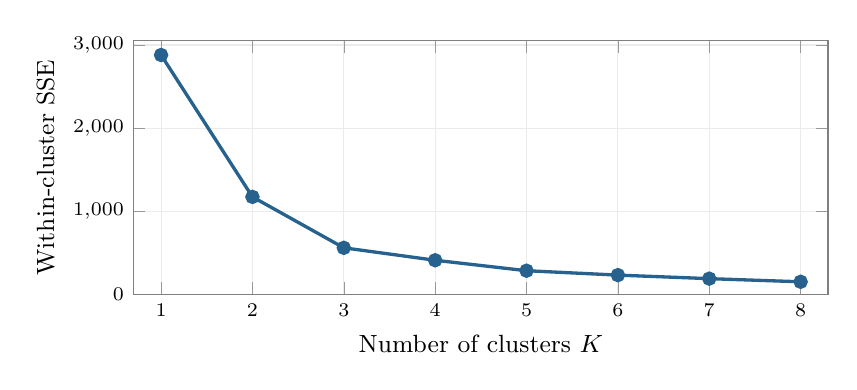
\begin{tikzpicture}
\begin{axis}[width=10.4cm,height=4.8cm,xlabel={Number of clusters $K$},ylabel={Within-cluster SSE},xmin=0.7,xmax=8.3,xtick={1,...,8},ymin=0,ymax=3050]
\addplot[very thick,cA,mark=*,mark size=2pt] coordinates {(1,2880.0000000) (2,1172.3675308) (3,559.3452698) (4,409.6251344) (5,283.7710163) (6,230.9242102) (7,188.3138578) (8,150.6052868)};
\end{axis}
\end{tikzpicture}
\end{center}
\small Here $K=3$ is a reasonable compact summary; $K=4$ refines it. An elbow is a judgment, not an automatic proof of the true number of groups.
\src{Same 2D standardized weather data for every $K$; best of 20 starts, seed 6021.}
\note{Have students compare the improvement from two to three with three to four. Do not compare these SSE values numerically to the 3D objective or to an unscaled run. Lower loss is meaningful only while the data representation stays fixed.}
\end{frame}

\begin{frame}{Silhouette: cohesion compared with separation}
For point $i$:
\begin{itemize}
\item $a(i)$: average distance to the \textbf{other points} in its own group.
\item $b(i)$: smallest average distance to the points in any other group.
\end{itemize}
\[
s(i)=\frac{b(i)-a(i)}{\max\{a(i),b(i)\}},\qquad -1\leq s(i)\leq1.
\]
\begin{itemize}
\item Near 1: relatively cohesive and well separated.
\item Near 0: groups overlap around this point.
\item Negative: another group is closer on average.
\end{itemize}
\begin{block}{Example}
If $a(i)=2$ and $b(i)=5$, then $s(i)=3/5=0.6$.
\end{block}
\src{Use ordinary Euclidean distances in the same standardized space. \href{https://scikit-learn.org/stable/modules/generated/sklearn.metrics.silhouette_score.html}{Silhouette documentation}.}
\note{These distances are point-to-point, not distances to the centroids. Negative does not mean misclassified against known truth. The average silhouette summarizes all points; singleton silhouettes are conventionally zero, and the measure is not defined for K=1.}
\end{frame}

\begin{frame}{Read diagnostics together, then inspect the groups}
\begin{center}
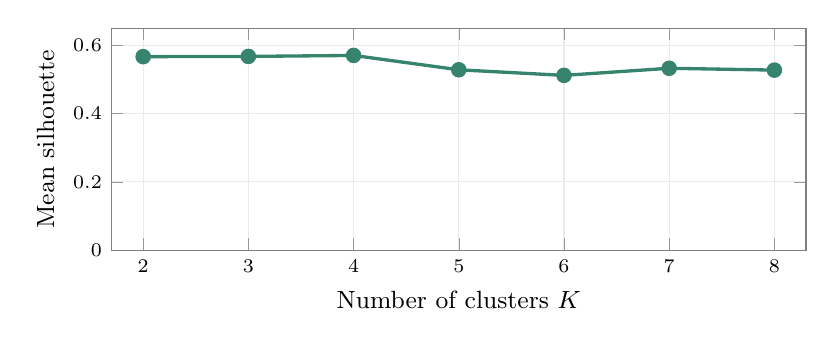
\begin{tikzpicture}
\begin{axis}[width=10.4cm,height=4.4cm,xlabel={Number of clusters $K$},ylabel={Mean silhouette},xmin=1.7,xmax=8.3,xtick={2,...,8},ymin=0,ymax=0.65]
\addplot[very thick,cC,mark=*,mark size=2.2pt] coordinates {(2,0.5667651) (3,0.5674235) (4,0.5703057) (5,0.5282405) (6,0.5118552) (7,0.5327057) (8,0.5273386)};
\end{axis}
\end{tikzpicture}
\end{center}
\small In this 2D snapshot, scores for $K=2,3,4$ are similar: approximately $0.567$, $0.567$, and $0.570$. A tiny improvement does not settle the substantive choice.
\begin{itemize}
\item Compare profiles and sizes; repeat across seeds and date windows.
\item A higher silhouette does not establish meteorological truth.
\end{itemize}
\note{This is a useful real example where the diagnostics are not a dramatic answer key. Temporal dependence means adjacent hours are related; a new date window tests robustness more honestly than treating every hour as an independent replication.}
\end{frame}

\begin{frame}{When should we question the result?}
\begin{itemize}
\item \textbf{Outliers:} squared distance gives extreme values large influence.
\item \textbf{Geometry:} elongated, curved, or differently dispersed groups may not fit nearest-center partitions well.
\item \textbf{Representation:} redundant features can count similar information twice.
\item \textbf{Weather sampling:} many dry hours, day/night effects, seasons, and adjacent-hour dependence affect what we see.
\item \textbf{Live refresh:} a new window changes the dataset, and potentially the clusters.
\end{itemize}
\begin{block}{A defensible analysis}
Explain the feature and scaling choices, inspect the profiles, examine stability, and report limitations with the grouping.
\end{block}
\note{KMeans always creates a partition when possible, even if there are no sharply separated natural groups. A log(1+precipitation) transformation is a possible sensitivity analysis, but changes the meaning of distance and of a back-transformed center. Keep it optional here.}
\end{frame}

\begin{frame}{Explain, interpret, and diagnose}
\begin{enumerate}
\item Why does the assignment step hold centers fixed?
\item Why does the update use a mean rather than an arbitrary point?
\item Can SSE stop changing even though another initialization gives a better result?
\item Why can adding precipitation change the cloud/humidity grouping?
\item What evidence would justify naming a cluster ``wet''? What would the name leave out?
\end{enumerate}
\begin{block}{Connection to modern data science}
The same reasoning applies to grouping customers, documents, sensor states, or learned embeddings: representation determines similarity, and clusters require interpretation.
\end{block}
\note{Use these as brief discussion prompts rather than a lengthy quiz. Expected answers should mention conditional minimization, squared error, local solutions, changed geometry, and inspection of distributions rather than only centroids.}
\end{frame}

\begin{frame}{Readings and companion materials}
\small
\textbf{Core reading}
\begin{itemize}
\item James, Witten, Hastie, Tibshirani, and Taylor, \emph{An Introduction to Statistical Learning with Applications in Python}: Sections 12.1, 12.4.1, and 12.4.3.\newline
\href{https://www.statlearning.com/}{statlearning.com}
\end{itemize}
\textbf{Computation and interpretation}
\begin{itemize}
\item Companion Colab notebook: inspect the data, fit KMeans, visualize groups, and compare $K$ and initialization.
\item \href{https://scikit-learn.org/stable/modules/clustering.html}{scikit-learn clustering guide} and \href{https://scikit-learn.org/stable/modules/generated/sklearn.cluster.KMeans.html}{KMeans API reference}.
\item \href{https://open-meteo.com/en/docs}{Open-Meteo weather variables and API documentation}.
\end{itemize}
\textbf{Optional deeper reading}
\begin{itemize}
\item Hastie, Tibshirani, and Friedman, \emph{The Elements of Statistical Learning}, Section 14.3.6 (K-means).\newline
\href{https://hastie.su.domains/ElemStatLearn/}{hastie.su.domains/ElemStatLearn}
\end{itemize}
\note{The main lecture ends here. The appendix supports questions about gap statistic, edge cases, mixed data, and alternative clustering methods. The notes and companion notebook use the same frozen weather dataset and explicit reference-fit settings.}
\end{frame}

\appendix

\begin{frame}{Optional: the gap statistic}
\small
Does the clustering improve on what we would expect from a reference dataset with no comparable group structure?
\[
\mathrm{Gap}(K)=\mathbb{E}^{*}[\log W_K^{*}]-\log W_K,
\]
where $W_K$ is the observed within-cluster dispersion and $W_K^*$ comes from reference datasets.
\begin{itemize}
\item Simulate reference datasets, often from a suitable uniform box.
\item Cluster each with the same method to estimate the expected log dispersion.
\end{itemize}
\begin{block}{Original selection rule}
Choose the smallest $K$ such that
\[
\mathrm{Gap}(K)\geq\mathrm{Gap}(K+1)-s_{K+1},
\]
where $s_{K+1}$ includes simulation uncertainty.
\end{block}
\src{Tibshirani, Walther, and Hastie (2001). \href{https://doi.org/10.1111/1467-9868.00293}{Estimating the number of clusters in a data set via the gap statistic}.}
\note{Avoid presenting the criterion as simply maximizing gap. The reference distribution matters. With B simulations, $s_k$ is the simulation standard deviation of log dispersion multiplied by sqrt(1+1/B). This material is optional, not an additional required diagnostic in the main lesson.}
\end{frame}

\begin{frame}{Optional: ties, empty groups, and stopping}
\begin{itemize}
\item \textbf{Tie:} assign to one center using a fixed convention.
\item \textbf{Empty group:} its mean is undefined. Keep the old center or reinitialize according to an explicit policy.
\item \textbf{Identical observations:} there cannot be more distinct positive-size geometric groups than distinct feature vectors.
\item \textbf{Stopping:} stable assignments, sufficiently small movement, or an iteration limit are different stopping criteria.
\end{itemize}
\begin{block}{For the reference tables in these notes}
We use zero tolerance ($\texttt{tol}=0$), at most 300 iterations per start, 20 starts, and seed 6021. The reported centers equal their final group means up to numerical precision.
\end{block}
\note{The dashboard's documented empty-cluster policy may differ from scikit-learn's. That can change paths without changing the conceptual assignment/update steps. A max-iteration stop should not be claimed as convergence. If tolerance ends a fit early, reported labels and centers can differ slightly from exact group means.}
\end{frame}

\begin{frame}{Optional: categorical features and Gower distance}
\begin{itemize}
\item Standard KMeans uses numerical coordinates, squared Euclidean distance, and arithmetic means.
\item A nominal label such as ``cloudy'' does not have a meaningful arithmetic mean.
\item Integer coding can create arbitrary distances. One-hot encoding changes the geometry and feature weighting.
\item Gower distance can combine appropriately scaled numerical and categorical comparisons, but it is not the standard KMeans objective.
\end{itemize}
\begin{block}{Connect to KNN}
KNN can use a chosen pairwise distance directly. KMeans also needs a compatible center and update rule. For general dissimilarities, consider methods such as K-medoids or suitable hierarchical clustering.
\end{block}
\note{This addresses the recent Gower discussion. Do not imply that swapping an arbitrary distance into KMeans preserves the mean update or its convergence argument. The weather code is intentionally excluded from the main feature set.}
\end{frame}

\begin{frame}{Optional: choosing another clustering approach}
\small
\begin{tabular}{L{2.1cm}L{3.7cm}L{4.1cm}}\toprule
Method & Useful perspective & A question to ask\\\midrule
KMeans & Summarize with $K$ numerical means & Are compact nearest-center groups useful?\\[0.5em]
Hierarchical & Build nested groupings with a linkage rule & Which distance and linkage express similarity?\\[0.5em]
Density based & Seek connected dense regions; may mark noise & What density scale and neighborhood are appropriate?\\[0.5em]
K-medoids & Represent groups by observed points & Is a general dissimilarity or an observed representative needed?\\\bottomrule
\end{tabular}
\vspace{0.8em}
\small Hierarchical behavior depends on linkage: Ward favors compact groups; single linkage can follow irregular shapes but may chain.
\src{\href{https://scikit-learn.org/stable/modules/clustering.html}{scikit-learn clustering guide}; ISLP, Section 12.4.2 (optional next topic).}
\note{This is orientation, not a second lecture. Avoid claiming that all hierarchical methods have flexible shape assumptions. Choice of representation and distance remains central across these approaches.}
\end{frame}

\end{document}
